%!TEX root = main.tex
%%%%%%%%%%%%%%%%%%%%%%%%%%%%%%%%%%%%%%%%%%%%%%%%%%%%%%%%%%%%%%%%%%%%%%%%%%%%%%%%%%%%%%%%%%%%%%%%%%%%%%
%
%   Filename    : chapter_3.tex 
%
%   Description : This file will contain your Theoretical Framework (Math equations, machine learning algorithms, and the such that will conclude in the realization of the most preferred concepts for constructing the system.
%                 
%%%%%%%%%%%%%%%%%%%%%%%%%%%%%%%%%%%%%%%%%%%%%%%%%%%%%%%%%%%%%%%%%%%%%%%%%%%%%%%%%%%%%%%%%%%%%%%%%%%%%%

\chapter{Theoretical Framework}

This chapter provides a thorough discussion of the different studies and theories behind the three main concepts of this study. The first few sections will tackle research on Human-Computer Interaction. The next set of sections will focus on User Experience Evaluation methods, and finally, Musical Composition and Metacreation. 

\section{Human-Computer Interaction}

	The study of Human-Computer Interaction (HCI) is about how technology can make an impact to human life \citep{dix2009human}. Its birth can be traced back to the studies of \citet{shackel1959ergonomics} and \citet{engelbart1962augmenting}. Both studies explored the approach of developing systems or interfaces for the benefit of the human intellect. This research stemmed from the increasing complexity of human tasks, and the need for technology to augment the capabilities of humans when performing these tasks \citep{engelbart1962augmenting}.
    
    HCI is multi-disciplinary, borrowing principles and theories from psychology, sociology, and computer science \citep{dix2009human, sinha2010human}. In HCI, one must learn to understand the users, which can be done through user observation or interviews, to develop systems and interfaces that would fit their backgrounds and needs \citep{fischer2001user}.
    
	One of the core topics in HCI is the issue of usability \citep{frokjaer2000measuring, dix2009human}. Usability tackles questions about effectiveness, efficiency, and satisfaction. Effectiveness asks if users can achieve their goals or perform their tasks properly and correctly when using the system \citep{frokjaer2000measuring}. Efficiency talks about whether users can perform the said goals with minimum use of resources or effort \citep{frokjaer2000measuring}. Finally, satisfaction is about finding out if users enjoy using the system or feel comfortable using it \citep{frokjaer2000measuring}. These usability issues can be achieved through the proper use of design principles (discussed in Section \ref{sec:designprinciples}).

    The growth of technological study and the emergence of new technological platforms brought with it new subfields under Human-Computer Interaction such as interaction design, user interface software technology, and user experience.
    
	\subsection{Interaction Design}
    
    Interaction functions as an essential factor to society's progress \citep{rogers2011interaction}. Humans interact with other humans or objects on a daily basis. These objects could be mobile phones, laptops, ATMs, and more. But not all of these have good usability or interaction. In that case, the interaction of these objects might not have been designed with the user in mind \citep{rogers2011interaction}. Even though these objects may be considered usable, they might not provide the best user experience when being used. 
    
    The goal of interaction design is to lessen these bad experiences when using objects, or in this case, technology \citep{shedroff1999information,rogers2011interaction}. User satisfaction is imperative to interaction design. It is about designing interactions that would not only benefit users, but would also reduce cognitive load and make the experience enjoyable or pleasurable \citep{tidwell2010designing}. 
    
    The continued study of interaction design allowed researchers and designers to identify a set of design principles. These principles serve as guidelines to designing good interactions and interfaces \citep{rogers2011interaction}. 

	\subsubsection{Design Principles}
    \label{sec:designprinciples}
    
    	What most developers or software development companies forget is that it is not always about how aesthetically pleasing the product is, rather, it is about how functional and easy it is for users of varying experience to understand how to use it \citep{blair2008user}. The overall system design should incorporate both functionality and visual appeal to provide value to its users.
        
        According to \citet{blair2008user}, the goal of the software should be decided and set at the start so that the interface is designed to support that goal. The design should make it obvious what the goal is all about. However, this should not make the design any less aesthetically pleasing. The designer should keep in mind what the software aims to do as well as making it pleasing for users to view and use. 
        
        Developers and designers should work together to form the design and user interface of the system. According to \citet{galitz2007essential}, the interface is the most important part of the system because it is what the users could see and interact with all the time. A testament to this importance is the finding that good design could help users become more productive and reduce cognitive load by up to 40\% \citep{galitz2007essential}. 
        
        Similarly, it was found in the study of \citep{cope1995cost} that redesigning just one web page to follow good design standards allowed a company to cut costs by \$20,000. This redesigned web page increased user productivity and reduced user error and training time. 
        
        \citet{mandelbaum2014design} notes four key principles to consider when designing products and interfaces (see Table \ref{tab:key-design-principles}):
        
        \begin{longtable}{|p{2cm}|p{11.6cm}|} 
        \caption{Key Design Principles} \label{tab:key-design-principles} \\
        \hline
        
        	Design Principle & Description \\ \hline
            
            Axis & The Axis, is an imaginary line that arranges, and aligns elements \citep{mandelbaum2014design}. It is considered as the most basic of the principles, but is equally important. When objects in an interface fall in or follow one axis, the design would give the impression of order. The axis allows movement in a straight line that the user's eyes can follow \citep{mandelbaum2014design}. The axis directs users towards something in the design. \\ \hline
        
        	Symmetry & The second principle, Symmetry, works together with the axis to promote balance \citep{mandelbaum2014design}. Symmetry enables balance between both sides of the axis, aligning and making both sides of an interface similar. Having symmetry gives users the feeling of harmony, and even the slightest difference in alignment or order can throw of the balance of a design and give a feeling of discomfort \citep{mandelbaum2014design}. \\ \hline
        
        	Hierarchy & Hierarchy is about showing the importance of certain elements in a design \citep{mandelbaum2014design}. One example of this is making one article in a news feed larger than the rest. The larger article would catch the users attention first and give the impression that it is more urgent or important compared to others. Other ways to show hierarchy could be through its placing or its shape. \\ \hline
        
        	Rhythm & Lastly, Rhythm, denotes patterns in the design. Having rhythm in the design allows users to find patterns and better recognize and know where to look for particular information \citep{mandelbaum2014design}. This can be seen in a Twitter feed where a list of tweets would look the same, helping users where to find the like button, or the user's twitter handle, etc. \\ \hline
           
        \end{longtable}
        
        Although they are not solid rules, these principles can be considered as building blocks that can be used to build an interface. The design is considered as the most important element of the system because it is what user can see and interact with \citep{galitz2007essential}.. Thus, careful consideration should be put in an application's overall design.
        \begin{comment}
        
        
        \begin{itemize}
        	\item Axis
            \item Symmetry
            \item Hierarchy
            \item Rhythm
\end{itemize}
        
        The axis, is an imaginary line that arranges, and aligns elements \citep{mandelbaum2014design}. It is considered as the most basic of the principles, but is equally important. When objects in an interface fall in or follow one axis, the design would give the impression of order. Additionally, the axis allows movement since it is a straight line that the user's eyes can follow \citep{mandelbaum2014design}. This movement can be used to direct users towards something in the design.
        
        The second principle, symmetry, works together with the axis to promote balance \citep{mandelbaum2014design}. Symmetry means balancing both sides of the axis, meaning both sides of an interface should be similar, and aligned. Having symmetry gives users the feeling of harmony, and even the slightest difference in alignment or order can throw of the balance of a design and give a feeling of discomfort \citep{mandelbaum2014design}.
        
        Hierarchy is about showing the importance of certain elements in a design \citep{mandelbaum2014design}. One example of this is making one article in a news feed larger than the rest. The larger article would catch the users attention first and give the impression that it is more urgent or important compared to others. Other ways to show hierarchy could be through its placing or its shape.
        
        Lastly, rhythm, denotes patterns in the design. Having rhythm in the design allows users to find patterns and better recognize and know where to look for particular information \citep{mandelbaum2014design}. This can be seen in a Twitter feed where a list of tweets would look the same, helping users where to find the like button, or the user's twitter handle, etc. 
        
        Although they are not solid rules, these principles can be considered as building blocks that can be used to build an interface. Again, careful consideration should be put in the design because it is considered as the most important element of the system because it is what the users can see and interact with \citep{galitz2007essential}.
        
        \end{comment}
        
	\subsubsection{Information Design}
    
		Communication is an essential aspect of the everyday lives of people. In businesses, it is important that they are able to communicate and get the point across to their clients and consumers. To do this, information must be designed in a way that can easily and efficiently be used and understood by people. This is where the art of information design comes in \citep{horn1999information}.
        
        An integral part of interaction design, information design involves analysis and understanding of not only the content of the message or information, but how it will be presented as well \citep{pettersson2002information}. It is about how to clearly communicate or send across information which is a key aspect in designing a good interaction \citep{shedroff1999information}.
        
        It is with proper organization that good information design is achieved, which can also lead to good interaction design \citep{shedroff1999information}. Information can be organized in several ways such as: alphabet, location, similarities, and more. Organizing these in such a way allows users to better understand and connect the individual piece of information \citep{shedroff1999information}. Additionally, \citet{blair2008user} advises the use of visualizations such as charts or graphs when presenting large information in order to make it easier for people to digest the information. 
        
        Even though information design is its own discipline, it should still follow the common design principles so that the information can be presented neatly and effectively \citep{shedroff1999information}. The information, or the way it is presented, is still a part of the overall design of the system so similar to designing an interface, it is good practice that designers keep in mind the goal of the system when trying to formulate how the information will be presented. 
        
        Going back to the hierarchy principle, the most important information should be presented in a way that would easily grab a user's attention like making it larger than the others or placing it at a position that can easily be seen \citep{mandelbaum2014design}. This just goes to show that the design principles mentioned above encompass all kinds of design, from visual design to information design.

	\subsubsection{Input and Interaction}
    	
        Without humans, there would be no technology \citep{commoner2014closing}. Despite machines being more computationally powerful and efficient, there is still a need for human input. Because of the emergence of several machines for daily use, different input methods have been developed. 
        
        For computers, there was the mouse, keyboard, tablet, and trackball, with the mouse and keyboard being the most popular \citep{engelbart1968a, mackenzie1991a}. With the rise in popularity of mobile phones, users can now interact with touch screens through gesture interactions \citep{chen2014agraph}. As such, these methods of input will be further discussed in the next few chapters.
    
    % add opener

		\paragraph{Traditional Computer Input}
        
      	During the advent of the computer becoming a consumer product, the keyboard and mouse were present to accompany the Windows, Icons, Menus, and Pointing Devices (WIMP) interaction style \citep{porta2007human}. The keyboard and mouse were also innovations during their time. Both were used to test how new kinds of interaction between a human and computer could augment the overall output of a computer user \citep{engelbart1968a}. 
        
        %As such, this section will discuss how each of these input devices have affected or furthered the progress of Human-Computer Interaction during their time.

Keyboards were mainly used to type commands into a computer device to fulfill a task the user would like to do \citep{karat1986a}. In the earlier times, keyboards were used alongside a command line interface, which made up most of the interaction during the time where graphical user interfaces were yet to be known \citep{galitz2007essential}. The keyboard is usually accompanied by a mouse where they are used in conjunction to perform tasks with computers \citep{engelbart1968a}. There have been events to also increase the comfort of using the keyboard to create less strain on the wrists or arms of the user \citep{grant1994computer}.  

            %Keyboards were mainly used to type commands into a computer device to fulfill a task the user would like to do \citep{karat1986a}. In the earlier times, keyboards were used alongside a command line interface, which made up most of the interaction during the time where graphical user interfaces were yet to be known \citep{galitz2007essential}. The keyboard's keys can also be used to navigate menus that are designed to be traversable through specific keys on the keyboard. The keyboard is usually found in a workstation accompanied by a mouse or pointer for both their features to be used in conjunction with a computer in hopes to fulfill tasks quicker \citep{engelbart1968a}. There have been events to also increase the comfortability of using the keyboard to create less strain on the wrists or arms of the user \citep{grant1994computer}.  

The mouse is a commonly used tool for navigating a 2D space in a computer screen \citep{engelbart1968a}. A standard mouse has three (3) buttons that can be used to select or perform additional tasks on the computer. Other devices were also built to navigate a 2D space, but the mouse was found to be the best performer among these devices \citep{karat1986a}

            % The mouse was found to be the faster way compared to other devices like light pens or joysticks when navigating a 2D space in the screen of a computer \citep{engelbart1968a}. A standard mouse can have 3 buttons mainly to be used when a user is ready to select whatever is pointed by the pointer on the computer screen. There are also devices that can be used to navigate the 2D space but it was found that the mouse performed the best during tests \citep{karat1986a}.

		% Add more
        
        	These traditional methods of input are commonly used in musical composition applications like Finale or Sibelius. In these applications, users usually input notes or modify the composition through a series of mouse clicks, while the more experienced users perform keyboard shortcuts \citep{knoder2017sibelius,knoder2017finale}. These methods can be efficient and easy, however the main drawback of these is that the keyboard and mouse are not easily portable, and are definitely not natural \citep{norman2010natural}.

		Touch-based interfaces were introduced at a later time to complement touchscreen devices and were meant to take advantage of the natural way humans interact. This was another step into finding out ways to improve the interaction between a human and a computer \citep{travis2014comparative}. 
       
        
		\paragraph{Gestural Interaction}

The goal of Human-Computer Interaction is to allow humans to interact with machines or computers naturally and seamlessly \citep{hasan2012human}. There is an increase in the use of gestures as a method of interaction in hand-held touch devices like tablets and smart phones and this is mainly attributed to gestures being considered as an an easy and natural method of interaction between humans and computers, compared to the use of a mouse or a stylus \citep{kurtenbach1996gestures, pavlovic1997visual, hasan2012human}. 

As most gestures found in gesture interaction systems are based on semiotics, \citep{muntigl2004modelling,radford2009introduction, kammer2010towards}, it is important to understand how gestures play a part in communication.

The work of \citet{wesp2001gestures} supports the idea that gestures help maintain spatial imagery. The use of gestures in communication helps in word retention because it builds up an idea through its perceivable signs \citep{krauss1998why}. This also applies to touch gestures since they build up perceivable actions that denote specific functions which make them an intuitive and natural way of interaction \citep{rautaray2015vision}.

In the study presented by \citet{roth2001gestures}, a gesture can be defined using four characteristics. The first characteristic of a gesture is that it moves from a resting position to a non-resting position and then back to a resting position. The second, \textit{stroke}, defines the peak structure of the gesture where it denotes the function of the gesture movement. The third, \textit{preparation} and \textit{recovery} phase, is when the stroke goes back to its resting position. The fourth characteristic is that it is symmetrical.

Recent studies on gestures led to its taxonomy wherein they are are classified based on their functions or how they were modeled \citep{roth2001gestures}. There are four classifications of gestures according to \citet{mcneill2007hand} (see Table \ref{tab:classifications-of-gestures}):

\begin{longtable}{|p{3cm}|p{10.6cm}|}
\caption{Classifications of Gestures} \label{tab:classifications-of-gestures} \\
\hline

Gesture & Description \\ \hline

\textit{Beats} or \textit{Batons} & These are gestures that do not express opinions. They are simple gestures which include slight movement of hands such as tapping or flicking that express responsiveness. \\ \hline

\textit{Deictic} gestures & These gestures attribute a contextual meaning such as pointing or extending of arms or hands. They are commonly used in referring to people or referring to locations. \\ \hline

\textit{Iconic} gestures & Iconic gestures use hand movements which relate to concrete objects.  \\ \hline

\textit{Metaphorical gestures} & These are movements that relate to a certain concept and makes a visual reference to it. An example would be a professor telling the class about the destruction of the world while closing his hands slowly. \\ \hline

\end{longtable}

% The first type, \textit{beats} or \textit{batons}, are gestures that do not express opinions. They are simple gestures which include slight movement of hands such as tapping or flicking that express responsiveness. The second type of gesture, \textit{deictic} gestures, are gestures that attribute a contextual meaning such as pointing or extending of arms or hands. They are commonly used in referring to people or referring to locations. The third type, \textit{iconic} gestures, are gestures that use hand movements which relate to concrete objects. The fourth type, metaphorical gestures, are movements that relate to a certain concept and makes a visual reference to it. An example would be a professor telling the class about the destruction of the world while he is closing his hands slowly.
        
			\subparagraph{Touch Gestures}        

Touch gestures have been widely used in recent years because of its intuitive and convenient nature \citep{chen2014agraph}. Some commonly used gestures in touch screen devices are pinching, scrolling, and tapping. There are three different types of touch-based interactions. The first one, raw ink, records the freehand drawing of the user. Sketching applications such as Paint is an example that uses this type of touch interaction. The second one, direct manipulation, is used in manipulating the user interface and gives real-time feedback to the user such as zooming and scrolling. The third one, indirect command, treats gestural input as a shortcut function in an application such as undo, redo, copy, and paste \citep{chen2014agraph}. In this study, direct manipulation will be used as the primary type of touch interaction for metacreation and other functionalities. 
            
The work of \citet{chen2014agraph} presents a way to recognize multi-touch gestures and assign specific functions for each with the use of graph modeling. In order to do so, it is important first to discern the difference between direct manipulation and indirect command. Direct manipulation calculates the position between fingers and it gives continuous feedback to the user while performing a gesture. For example, the act of pinching to zoom out a text document requires the system to continuously change the view in sync with the pinching motion. Indirect command, on the other hand, is concerned with the motion's shape and trajectory right after when the user performed a gesture. It captures the shape of motion after it has been performed and executes the assigned function. 

There are three types of information that needs to be considered when modeling a multi-touch gesture \citep{chen2014agraph}. The first one, spatial, stores the position of each gesture trail relative to each other. The second one, temporal, stores the order of trails and their corresponding duration. The third one, shape information, stores the shape of each trail which allows the system to distinguish the difference between a straight line swipe from a curve swipe.

Each gesture trail can be represented by three vertices in a graph \citep{chen2014agraph}. The first vertex, ($V_b$), represents the begin vertex. The second vertex, ($V_s$), represents the stroke vertex, and the third vertex, ($V_e$), represents the end vertex. Temporal and spatial information are represented using the following edges: $E_s$(x, y), $E_{st}$(x, y, t), and $A_{st}$(x, y, t), wherein subscripts s and st indicate whether an edge represents only spatial, or both spatial and temporal, respectively. Consider the following example in Figure \ref{fig:spatial-temporal-graph}:

\begin{figure}[H]
	\centering
	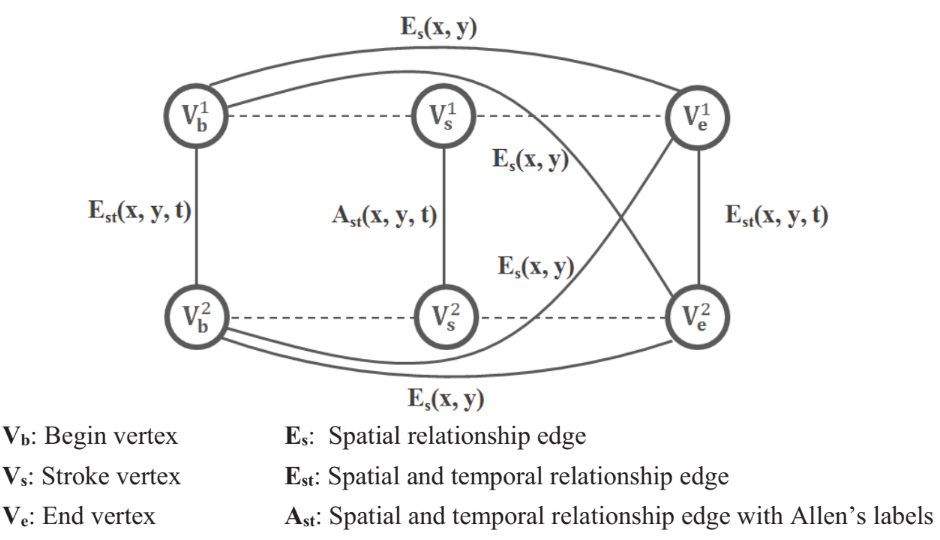
\includegraphics[scale=0.5]{SpatialTemporalGraph}
    \caption{An example of a two strokes gesture graph \citep{chen2014agraph}.}
    \label{fig:spatial-temporal-graph}
\end{figure}

In order to complete the information of the edges in Figure \ref{fig:spatial-temporal-graph}, Allen's relations that use discrete labels of time will be used as shown in Figure \ref{fig:allen-relations}.

\begin{figure}[H]
	\centering
	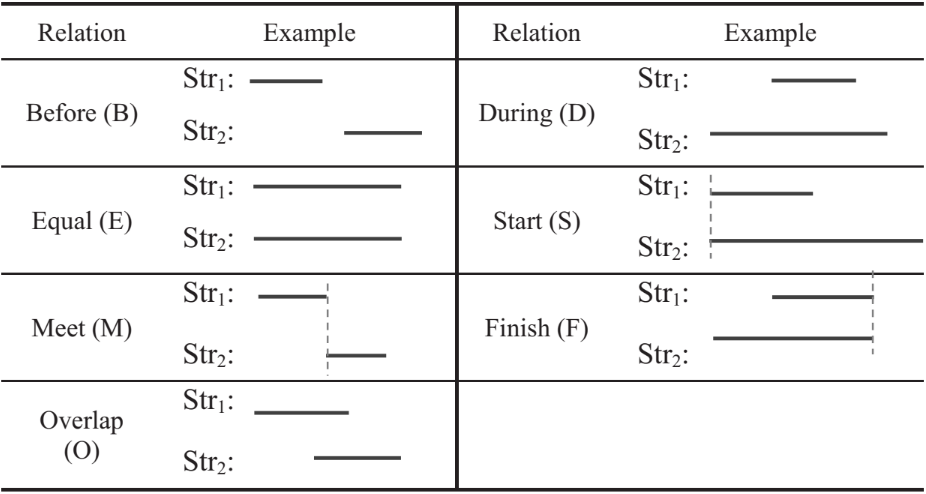
\includegraphics[scale=0.5]{AllenRelations}
    \caption{Examples of Allen's relations \citep{allen1983maintaining, chen2014agraph}.}
    \label{fig:allen-relations}
\end{figure}

In general, labeling the edges results in two possible cases:

\begin{enumerate}
\item \textit{Edges between stroke vertices ($A_{st}$)}: This represents the measurement and relationship of strokes with regards to time, x-axis, and y-axis. 
\item \textit{Edges between extremity vertices ($E_s$ and $E_{st}$)}: This represents the touching and lifting of fingers in a touch screen and so it only encompasses \textit{Equal} property for the time \textit{(E\_T)}, x-axis position \textit{(E\_X)}, and y-axis position \textit{(E\_Y)} in defining the edges between vertices.
\end{enumerate}


Shown in Figure \ref{fig:flick} is a flick gesture with its corresponding spatial relation and time duration. According to the relations of \citet{allen1983maintaining}, the flick gesture has an \textit{Equal\_X (E\_X)} and \textit{Before\_Y (B\_Y)} labels which denote that the x-coordinates of both strokes are equal and the y-coordinate of the first stroke is above (Before) the y-coordinate of the second stroke. The time duration is labeled as \textit{Equal\_T (E\_T)} to denote that the strokes were simultaneously performed. This results into edge \textit{$A_{st}$} having an equation: $A_{st}$(x, y, t) = \{E\_X, B\_Y, E\_T\}

\begin{figure}[H]
	\centering
	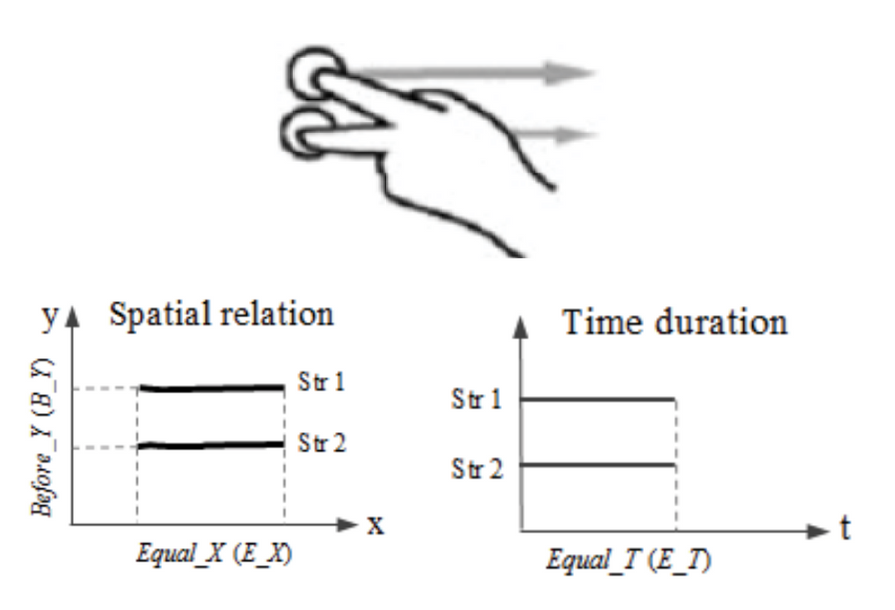
\includegraphics[scale=0.4]{flick_gesture}
    \caption{Flick gesture \citep{chen2014agraph}.}
    \label{fig:flick}
\end{figure}

\begin{comment}
\begin{figure}[H]
	\centering
	\includegraphics[scale=0.6]{Flick}
    \caption{Flick gesture \citep{chen2014agraph}}
    \label{fig:flick}
\end{figure}

\begin{figure}[H]
\centering
\begin{minipage}{.4\textwidth}
	\centering
	\includegraphics[width=.7\linewidth]{SpatialRelation}
    \caption{}
    \label{fig:spatial-relation}
\end{minipage}
\begin{minipage}{.4\textwidth}
	\centering
	\includegraphics[width=.7\linewidth]{TimeDuration}
    \caption{}
    \label{fig:time-duration}
\end{minipage}
\end{figure}
\end{comment}
In the graph of the flick gesture, the label $E_{st}$=\{E\_X, E\_T\} at the left and right side denote that the x-coordinates of both strokes are in the same region and they were performed at the same time. The label $E_{st}$=\{E\_Y\} on the top and bottom of the graph denote that both strokes were performed in the same region of the y-coordinate.

\begin{figure}[H]
	\centering
	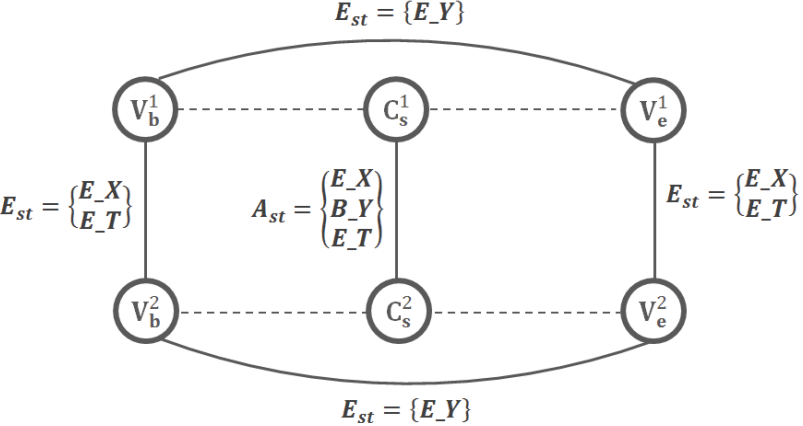
\includegraphics[scale=0.5]{FlickGraph}
    \caption{Flick graph \citep{chen2014agraph}.}
    \label{fig:flick-graph}
\end{figure}

In the application's selected platform, iOS, gestures are recognized through the \texttt{UIGestureRecognizer} class, implemented in the Swift programming language. This class is the one that detects gestures and passes them to other related objects that would act on that gesture. An important thing to note is that it does not perform anything related to the gestures, it only passes them. This was done in order to decouple the logic for recognizing the gesture and acting on it \citep{apple2017ui}.

By default, the \texttt{UIGestureRecognizer} class allows the detection of common gestures like taps, holds, pinchs, and more through its subclasses \citep{apple2017ui}. It communicates with \texttt{UIGestureRecognizerDelegate} classes to better control gestures in applications. The way gestures work in iOS is that the window or view reads the gestures and checks if any \texttt{UIGestureRecognizer} object recognizes the gesture performed. If one does, it would then pass control to that object \citep{apple2017ui}. 

	\subsection{User Interface Software Technology} 
    \label{sec:uist}
		
        With the large, yet still growing number of applications and software available in the market today, it is becoming increasingly hard for developers to make their application stand out. One important factor that decides an application's fate in the market is design \citep{deka2016datadriven}.

		Application design is a process \citep{curtis1988field,humphrey1995discipline} that takes time and effort not only from designers, but from developers and researchers as well. They must identify how best to design the interface in a way that users would find intuitive and natural. This process involves research on the users' needs and behaviors and user experience validation through testing and heuristics \citep{deka2016datadriven}. 
        
        Jakob Nielsen presents set of usability heuristics to follow for interface design \citep{nielsen1990heuristic, nielsen1994usability, nielsen2013usability}:
        \begin{itemize}
        	\item Visibility of system status
            \item Match between system and the real world
            \item User control and freedom
            \item Consistency and standards
            \item Error prevention
            \item Recognition rather than recall
            \item Flexibility and efficiency of use
            \item Aesthetic and minimalist design
            \item Help users recognize, diagnose, and recover from errors
            \item Help and documentation
		\end{itemize}
		
        \textit{Visibility of system status} denotes that users should always be informed about what's currently happening in the system. For example, the application is loading, then it should show that it is loading and not just a blank screen so the user won't think that the application froze.
        
        \textit{Match between system and the real world} means that systems should follow what is natural to the user. It should speak in the user's same language, using words and icons that the user can understand. 
        
        The \textit{user control and freedom} heuristic simply means that the user should be able to easily undo or redo their state in case of a mistake. 
        
        \textit{Consistency and standards} denotes that there should be consistency in the words used and the design. The system should not make the user think whether two buttons with the same name do different things.
        
        \textit{Error prevention} is important so that there will not be a need for error recovery. It is better to prevent users from committing errors rather than forcing them to recover from an error they made.
        
        \textit{Recognition rather than recall} should be kept in minding when designing a user interface to help reduce the cognitive load of users when using the system. Objects or icons should be clearly visible and easily retrievable to users.
        
        \textit{Flexibility and efficiency of use} means that the system should be more flexible to allow experienced users to speed up interaction or use shortcuts. 
        
        Systems should have \textit{aesthetic and minimalist design} that only shows relevant information to the user. This is so that the screen clean and reduce the cognitive load of the user. 
        
        Systems should \textit{help users recognize, diagnose, and recover from errors} through information that could easily be read and understood.
        
        \textit{Help and documentation} should also be included in the case that users would want to understand how to use the system better.
    

\section{User Experience Evaluation}

		User experience plays a key role in software development as it can drastically increase a product's return of investment \citep{bellamy2011deploying}. Usability allows the discovery of problems sooner which may save a lot of budget costs and may improve sales. Producing applications that are usable is often difficult to pull off in actual practice because of its iterative process which uses human observation and analysis. This implies that there are biases in terms of testing and analysis \citep{bellamy2011deploying}. Over the years, multiple solutions for user experience evaluation have been proposed.

	\subsection{Quantitative Evaluation}
    
    	\subsubsection{KLM-GOMS}
        	
            One example of a quantitative method for analyzing the usability of an application is by using \textit{cognitive modeling}, an analytic technique that measures the motor operations performed by the user with regards to the brain \citep{sauro2009estimating}. An example of this is measuring how fast a user can navigate an interface or interact with it. 
            
            The most commonly used cognitive modeling technique is GOMS, which stands for Goals, Operators, Methods, and Selection Rules. GOMS is a set of models for analyzing human-computer interaction and for removing user actions which are deemed useless or unnecessary \citep{card1983the}.
            
            One such example of a GOMS technique is the Keystroke Level Modeling (KLM) technique \citep{sauro2011measuring}. It is commonly used by practitioners due to its simplicity. The KLM technique is used to estimate user actions such as pointing, clicking, typing, and thinking \citep{sauro2009estimating}. The technique simply counts the number of operations it would take a user to achieve a certain goal or navigate a system. From there, ideas can be gained from where the users experience pain points when using the system. 
       
    	\subsubsection{Fitts' Law}
        
    		Another, and more descriptive method of analyzing usability is the Fitts' Law. Fitts' law is a predictive model for human movement that takes into account the distance from the target and the time it took the user to navigate to that target \citep{mackenzie1992fitts}.
            
            Fitts' Law was conceived from information theory, specifically that of Shannon's Theorem 17 (Equation \ref{eq:shannon}), which denotes the information capacity (\begin{math}C\end{math}), or the amount of information that can be sent, using a signal power (\begin{math}S\end{math}) within a specified bandwidth (\begin{math}B\end{math}), while affected by noise (\begin{math}N\end{math}) \citep{mackenzie1992fitts}.
            
            \begin{equation}
            	\label{eq:shannon}
            	C = Blog_2 \frac{S + N}{N}
            \end{equation}
    
    		Although there was no direct mathematical relation of Fitts' Law to that of Shannon's Theorem, Fitts got the idea from the theorem of how information is processed through human channels when performing tasks \citep{mackenzie1992fitts}. He derived some of the elements of information theory to form what is now called Fitts' Law (Equation \ref{eq:fitts}), where the index of performance (\textit{IP}) can be derived by dividing the specified task's index of difficulty (\textit{ID} by the movement time (\textit{MT}) it took to perform the task. 
            
            \begin{equation}
            	\label{eq:fitts}
            	IP = \frac{ID}{MT}
            \end{equation}
            
            From this, Fitts Law can be used in domains like physical movement, or movement on a digital screen. Using Fitts Law, pain points can be identified, and interface elements that affect a user's effectiveness when performing tasks can be found \citep{mackenzie1992fitts}. 
            
            Fitts Law will be heavily used in the study to help the researchers identify these pain points in the design. It will provide a numeric measure on the effectiveness of a user interface, making it easier for the researchers to document and compare results between previous versions of the interface. The measurement of Fitts Law can be made easier through CogTool (to be discussed in Section \ref{sec:cogtool}), which will also be used in this study. 
            
    	\subsubsection{CogTool}
        \label{sec:cogtool}
        
        % User experience plays a key role in software development as it can drastically increase a product's return of investment \citep{bellamy2011deploying}. Usability allows the discovery of problems sooner which may save a lot of budget costs and may improve sales. Producing applications that are usable is often difficult to pull off in actual practice because of its iterative process which uses human observation and analysis. This implies that there are biases in terms of testing and analysis. Over the years, a solution was proposed.
        
        
        Although useful for quantitatively understanding the user experience of an application, both KLM and Fitts' Law require that the users being tested are observed in order to calculate the time and make estimates for both models. This poses a problem because it requires manual work and is repeated multiple times depending on the number of tests required. Having to manually make estimates for KLM and Fitts' Law can be tedious and prone to error \citep{sauro2009estimating}. However, IBM's solution for this problem is the implementation of an iterative and quantifiable method of testing and analyzing a product's usability through the software, \textit{CogTool}. 
         
         CogTool is similar to other prototyping tools like InVision, but is more powerful for quantitative evaluation. Once an application's interface has been set in CogTool, with the simple click of a button a cognitive model for evaluation will be generated. CogTool eliminates the need to manually calculate KLM or Fitts Law, making it easier to quantitatively evaluate a user interface \citep{bellamy2011deploying}. 
         
		It uses \textit{storyboards} that demonstrate the different tasks of a user \citep{bellamy2011deploying}. These storyboards serve as the user interface of the system that is being tested. Inside these storyboards are \textit{frames} that serve as the different states of the UI. Each frame may have \textit{widgets} which can be used by the user to interact with. The assigned action for each widget is called \textit{transition}. A sample storyboard is shown in Figure \ref{fig:cogtool}. The rectangles inside the storyboard are the frames. The orange area inside the frame is the widget. The arrow between the frames is the transition.
        
       % Having to manually make estimates for KLM and Fitts' Law can be tedious and prone to error \citep{sauro2009estimating}. However, IBM's solution for this problem is the implementation of an iterative and quantifiable method of testing and analyzing a product's usability through the software, \textit{CogTool}. CogTool is similar to a prototyping tool like InVision, but it is more powerful as it also analyzes the behavior of a user while interacting with the designed prototype. It uses \textit{storyboards} that demonstrate the different tasks of a user \citep{bellamy2011deploying}. These storyboards serve as the user interface of the system that is being tested. Inside these storyboards are \textit{frames} that serve as the different states of the UI. Each frame may have \textit{widgets} which can be used by the user to interact with. The assigned action for each widget is called \textit{transition}. A sample storyboard is shown in Figure \ref{fig:cogtool}. The rectangles inside the storyboard are the frames. The orange area inside the frame is the widget. The arrow between the frames is the transition.
        
\begin{figure}[H]
	\centering
	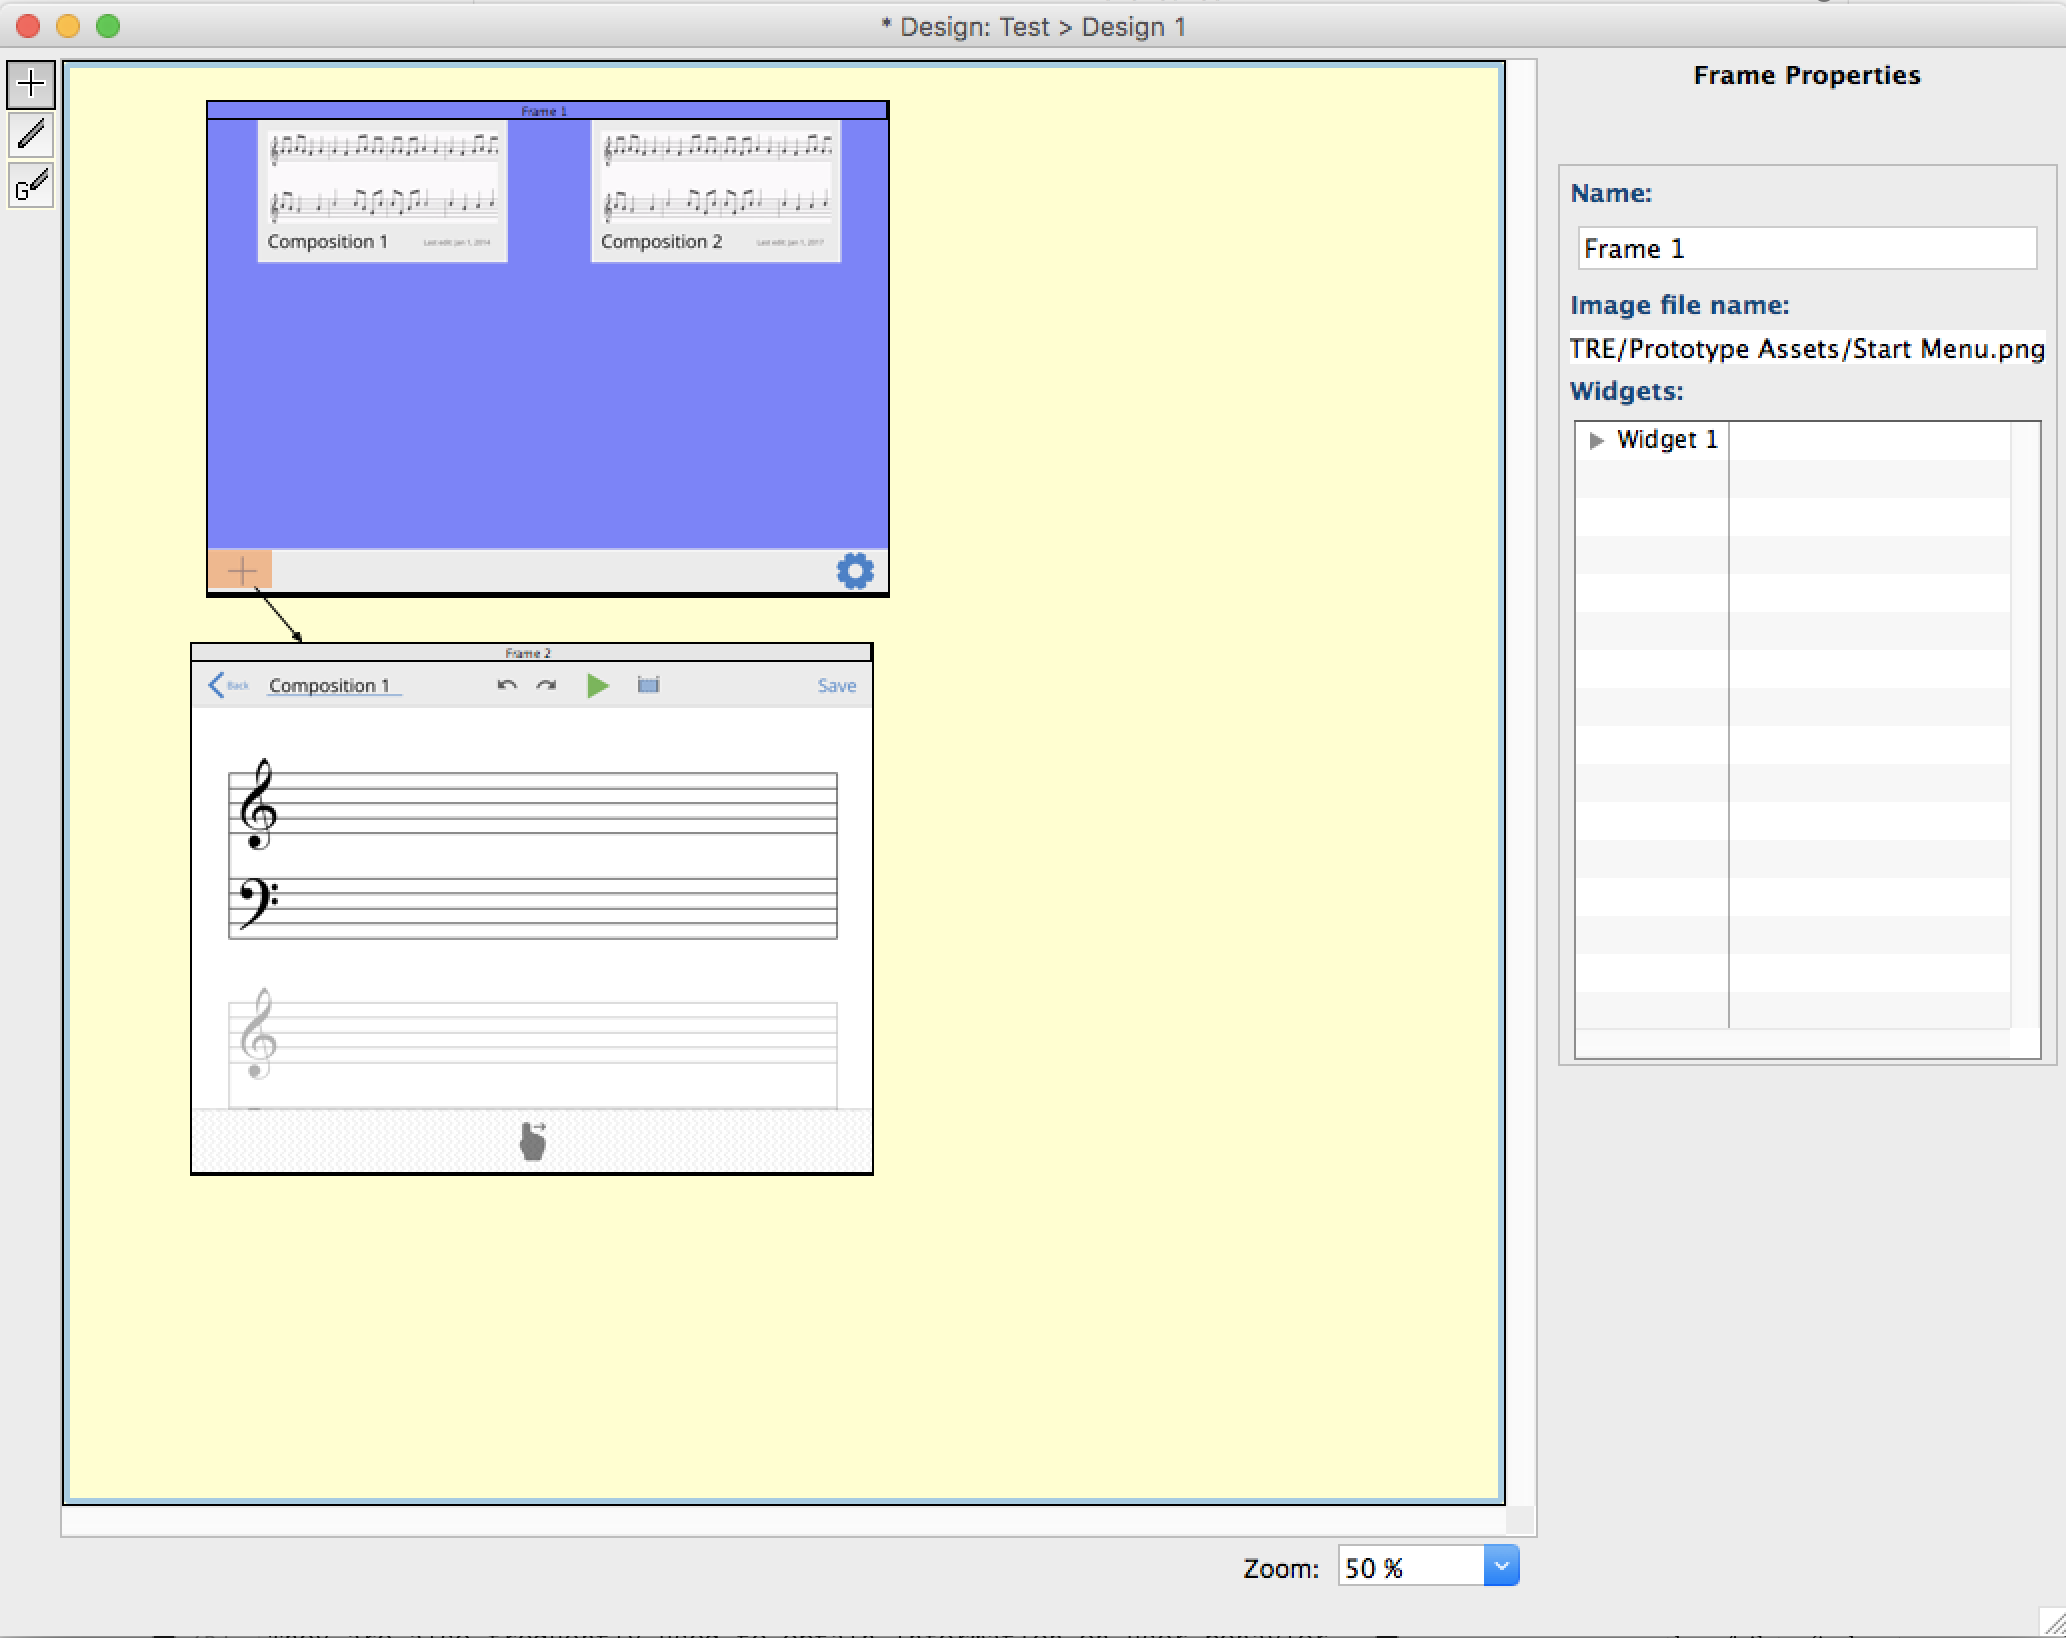
\includegraphics[scale=0.4]{CogToolMockup}
    \caption{CogTool storyboard of application mockup.}
    \label{fig:cogtool}
\end{figure}
        
        Once a storyboard has been setup completely, a starting frame must be chosen for the system to start with (see Figure \ref{fig:start-frame}).
        
\begin{figure}[H]
	\centering
	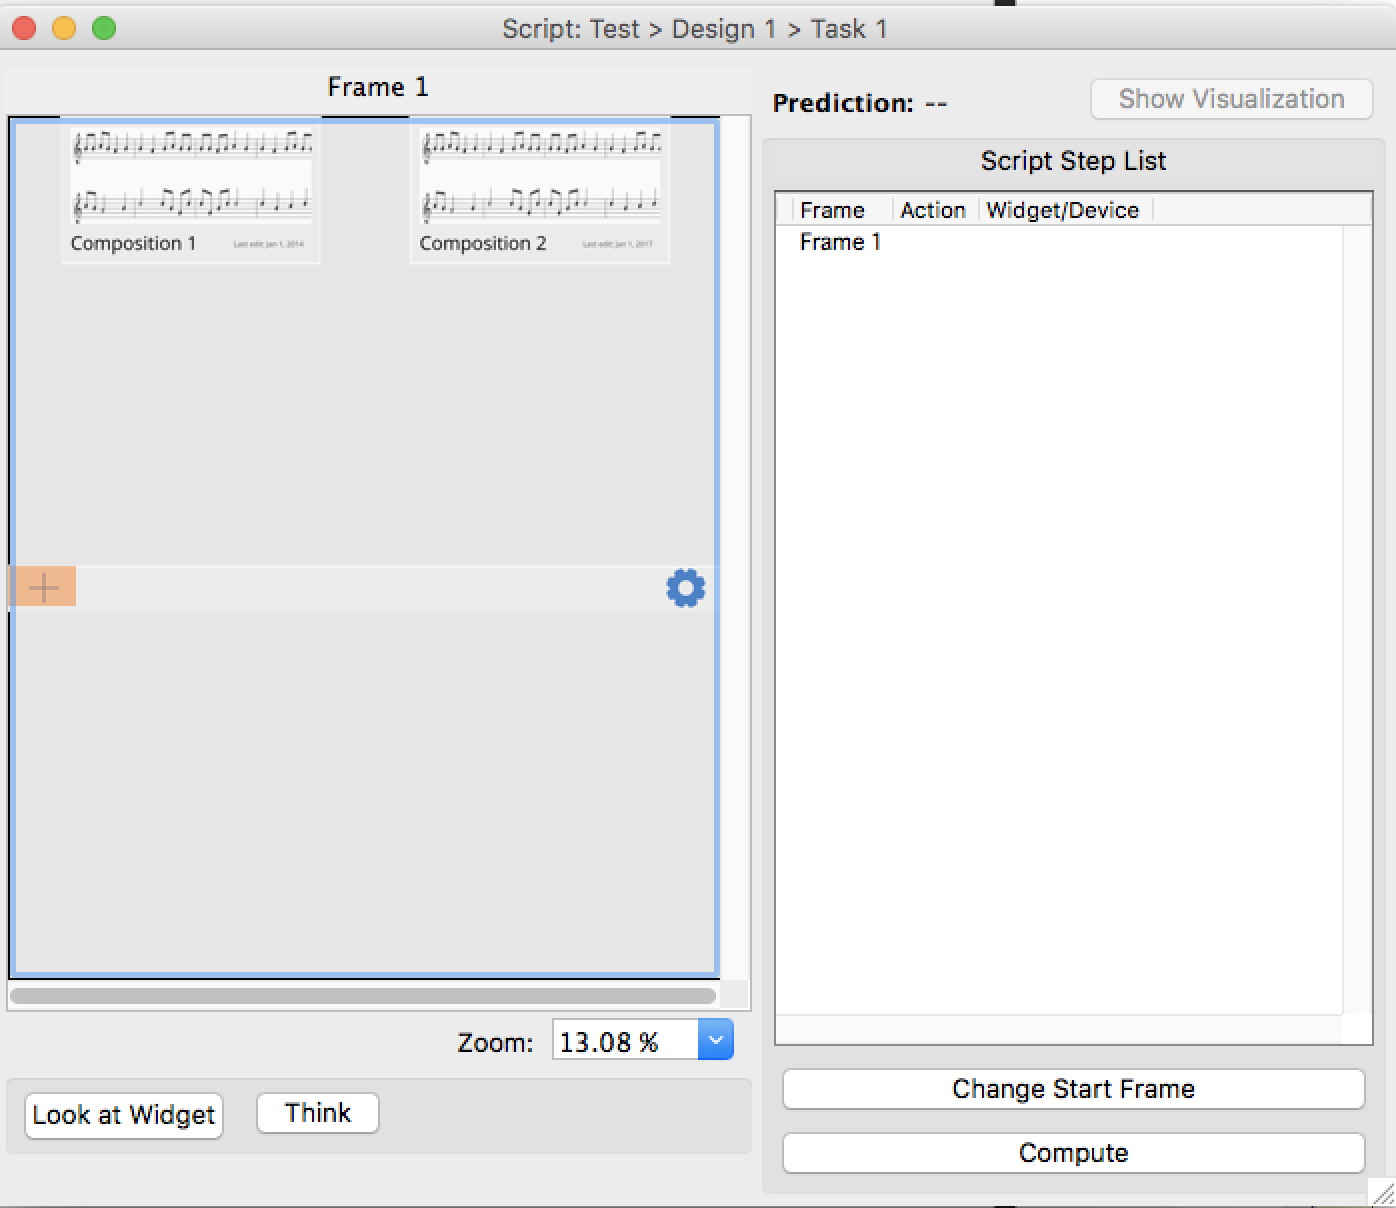
\includegraphics[scale=0.5]{StartFrame}
    \caption{Choosing a start frame for a storyboard.}
    \label{fig:start-frame}
\end{figure}
        
        CogTool has the ability to run an automated user that would go through the whole storyboard. The steps that the automated user takes will also be shown in the script step list (see Figure \ref{fig:script-step}). The list allows designers and analysts to easily identify what the user is doing and how long it takes the user to do it.
        
        % CogTool records all the actions performed by the user and it also records the idle times when the user is not doing any action. Figure \ref{fig:script-step} shows the script step list of CogTool where all the actions are shown while the user is interacting with the storyboard.
        
\begin{figure}[H]
	\centering
	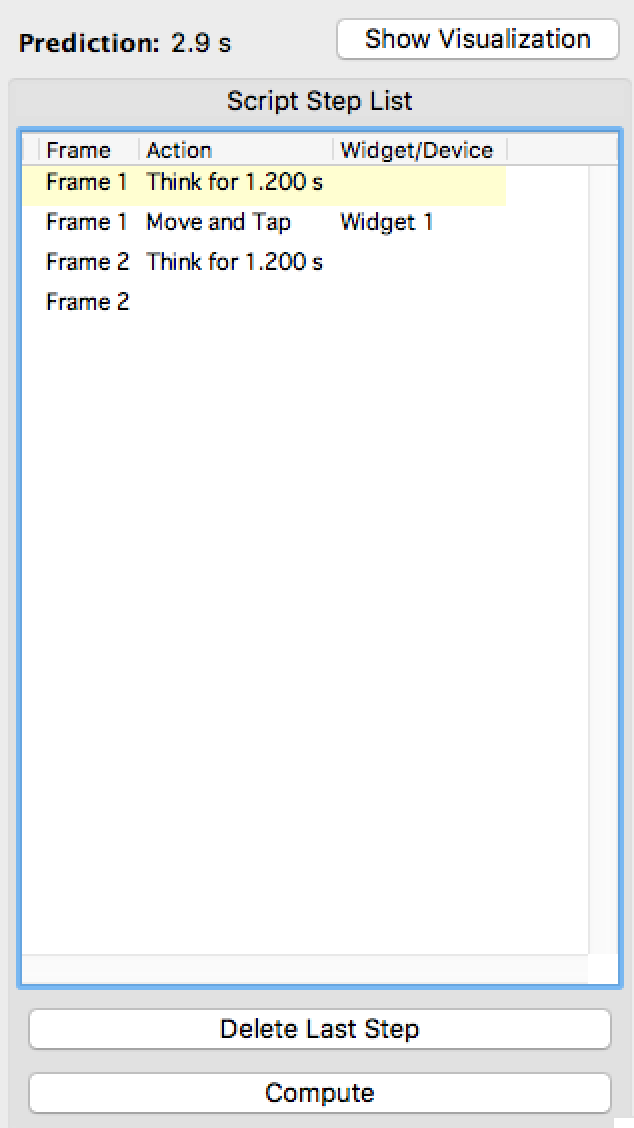
\includegraphics[scale=0.6]{ScriptSteps}
    \caption{Script step list of CogTool.}
    \label{fig:script-step}
\end{figure}  

When the user clicks on the compute button, CogTool computes for the estimate of the quantitative time of execution and visualization of timeline. The visualization shows the different tasks of the cognitive model on how it was able to derive the estimate (see Figure \ref{fig:cogtool-visual}).

\begin{figure}[H]
	\centering
	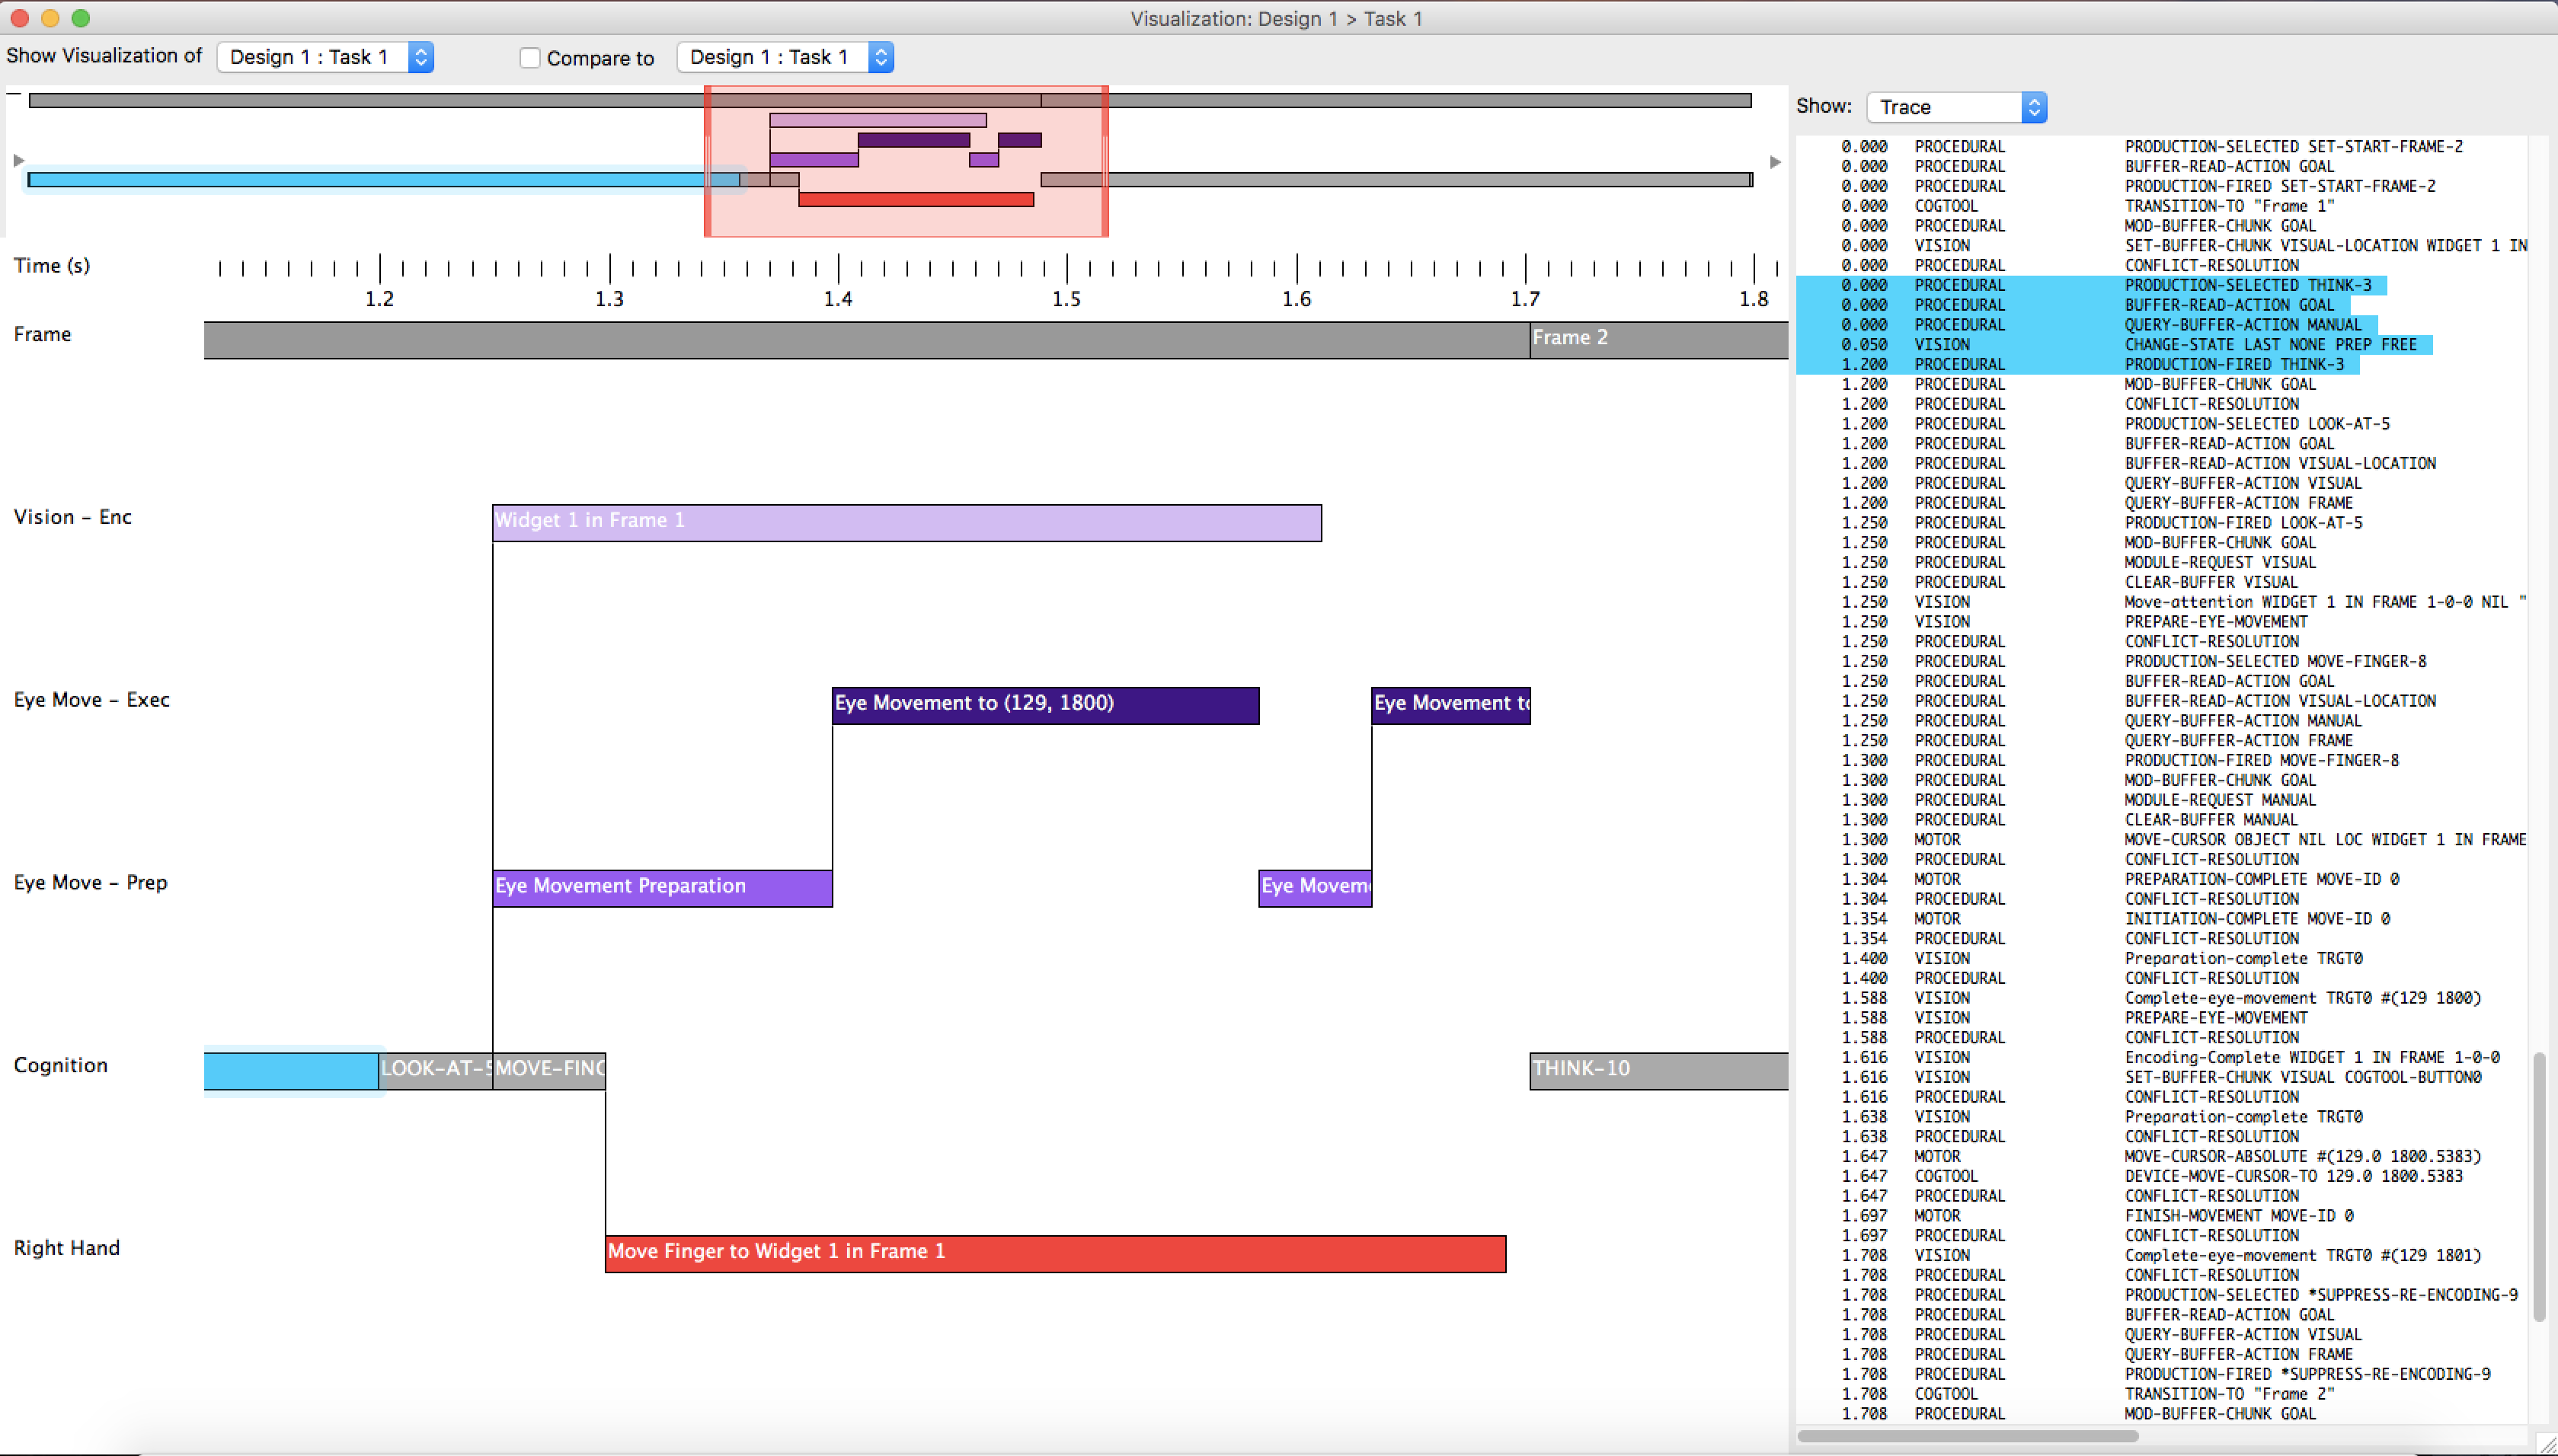
\includegraphics[scale=0.2]{CogToolVisualization}
    \caption{The highlighted part is the selected section of the user's action timeline.}
    \label{fig:cogtool-visual}
\end{figure}

The data presented by CogTool are useful for quickly evaluating the user experience of a system. It provides a quantitative model for analyzing the different tasks of a user and it can also be used for comparing different storyboards. This is helpful for designers to allow them to compare their design with competing designs \citep{bellamy2011deploying}.

% The data presented by CogTool are useful in evaluating the user experience of a system because it provides a quantitative model of analyzing the different tasks of a user and it can also be used for comparing different storyboards. This would be helpful especially for developers in determining whether a single line of code should already be written for an application based on the evaluated results.
        
        \subsubsection{Survey Instruments}

			Simple and easy to administer, surveys are one of the most commonly used methods of research \citep{goddard1996designing,mathers2007surveys}. Surveys can be used to gather information on individuals, given a set of questions. 
They are also frequently used to obtain information on user behavior and attitude \citep{mathers2007surveys}. Additionally, surveys may provide answers that may be generalized, depending on the way it was administered \citep{newsted1998survey}. 

		Surveys are good at finding out how many people do one thing or how many people think this way about something. However, they are limited in the sense that they fail to find out or answer why people do that one thing or why they think that way about something \citep{mathers2007surveys}. In cases like this, qualitative evaluation methods like focus group discussions are better at answering the ``why'' questions.
        
        Given that surveys are used to gather information on respondents' attitudes, several methods of measuring these have been developed. The most common one, however, is the Likert scale \citep{mcleod2008likert}. The Likert scale was developed by Rensis Likert in 1932 in order to provide a system for ``measuring'' the attitude of respondents. 
        
        Since then, the Likert scale has been commonly used as a five level scale measuring different levels of agreement or disagreement, frequency, importance, and likelihood on certain topics or concepts \citep{mcleod2008likert}. The advantage of this scale is that answers are not simply yes or no, and provide more insight on the attitude or behavior or the respondents \citep{likert1932technique,mcleod2008likert}.

	\subsection{Qualitative Evaluation}
    
		\subsubsection{User Acceptance Testing}
        
        The research will implement a mobile application for augmenting musical composition. To determine how effective the implementation of the system is, it will be tested on composers of varying skill. A method for getting feedback that would help identify issues in the application is User Acceptance Testing (UAT) \citep{davis2004toward}.
        
        %The research will implement a mobile application for augmenting musical composition. To determine how effective the implementation of the system is, it will be tested on composers of varying skill. A method to ensure that feedback is received that can be used to fix recurring issues or change any troubling detail in the application is through User Acceptance Testing (UAT) \citep{boltonuser}. 
        
        UAT can be used to measure the time it takes a user to finish a task, cognitive load, and their impression of the system after testing. These measures are seen in some experiments that performed user tests on similar systems like the touch-based system in the study of \citet{findlater2012beyond} where touch gestures and pop-up menus were the main features of the system. Music interaction research was also evaluated in the study of \citet{brown2017user} wherein it was found which factors were mostly used in testing, and how usability and aesthetics were the primary focus. These factors can be taken into consideration when planning the UAT for the system of the research.
        
        Before the UAT, there can be different tasks that can be designed for the user to accomplish based on the needs of the user. In evaluating music interaction research, \citet{brown2017user} enumerated the following categories of tasks given to participants:
        
        \begin{itemize}
        \item Specific Task
        \item Open Exploration
        \item Guided Exploration
        \item Watch Performance
        \item Prepare and/or Give Performance
        \item Workshop
        \item In The World Use
        \item Other
        \end{itemize}
        
        These categories can be used during the UAT of the system. There are also other concepts or methodologies that the group will consider when testing the system such as cognitive load through the use of CogTool, which was discussed in Section \ref{sec:cogtool}. These concepts can either be observed or used in conjunction with the UAT or they are implemented differently and individual from the UAT.
        
        	\paragraph{Think-Aloud Protocol}
            
            A concept that can be used during the UAT is the Think-Aloud Protocol. The Think-Aloud Protocol encourages the user to share their thought while performing tasks during the experiment. This protocol can help the user open up during the experiment and voice out whatever they are thinking whether it is their frustration with the system or their strategy when trying to complete a task \citep{gomoll1996some}. During testing, the user is reminded to constantly voice out their thoughts while completing tasks so that observations can include both actions and user motives \citep{gomoll1996some}. Although there is no specific standard followed by researchers in executing the Think Aloud Protocol \citep{mcdonald2013the,gill2012think}, there are still studies that provide guidelines such as the classical work of \citet{ericsson1998study} and augmented methods like the Explicit Think-Aloud (ETA) from the study of \citet{mcdonald2013the}.
            
            %A concept that can be used during the UAT wherein a user is encouraged to share their thoughts during the experiment is called the Think-aloud Protocol. This protocol can help the user open up during the experiment and voice out whatever their thinking whether its their frustration with the system or their strategy in trying to complete a task \citep{gomoll1996some}. During testing the user is reminded by the researchers to constantly voice out their thoughts while completing tasks so that observation can include both actions and user motives \citep{gomoll1996some}. Although there is no specific standard followed by researchers in executing the Think Aloud Protocol \citep{mcdonald2013the,gill2012think}, there are still studies that provide guidelines such as the classical work of \cite{ericsson1998study} and augmented methods like the Explicit Think-Aloud (ETA) from the study of \cite{mcdonald2013the}.
            
            In the work of \citet{ericsson1998study}, the Think-Aloud Protocol was mainly used during observation to detect problems as they occur. In this case, the information provided by the user must be validated due it being the user's own ideas and opinions \citep{ericsson1998study}. There are 3 guidelines provided in the study of \citet{ericsson1998study} to ensure the success of the Think-Aloud Protocol, these are: 
                       
            % In the work of \cite{ericsson1998study}, the Think Aloud Protocol was mainly used during observation to detect problems as they occur. Information provided by the user in this respect is important to be valid due to its nature of being from the introspection of the user \citep{ericsson1998study}. There are 3 classic guidelines provided by \cite{ericsson1998study} to ensure the validity of data verbalized by the user and to avoid the reactivity which can occur when any of these guidelines are violated. These guidelines are:
            
            \begin{itemize}
            \item A neutral instruction that does not request specific types of information
            \item A practice session
            \item A neutral ``keep talking'' reminder given by the researcher
            \end{itemize}
            
            The Think-Aloud Protocol was used in the study of \citet{yu2011probing} to better understand how students solve mathematical induction problems. These problems can be related to music as mentioned in the study of \citet{dorfler2001time}, where music has a complex set of features that are usually continuous in form. A musical composition can then be seen as a series of solutions to a mathematical problem. From this, the thought process of a composer can be captured using the Think-Aloud Protocol similar to the study of \citet{yu2011probing}.
            
            %The Think Aloud Protocol was used in the study of \citet{yu2011probing} to find out how a students solve mathematical induction problems specifically induction on infinite series. Using the Think Aloud Protocol \citeauthor{yu2011probing} was able to find more details of the students thought process while solving the problems. These problems can be related to music as mentioned in the study of \citet{dorfler2001time} wherein a complex set of features can be present within a composition usually infinite in form. This provides the relation of a composer composing music as a series of solutions as a mathematical problem as discussed by \citet{dorfler2001time} and the thought process of this problem solving by the composer can be captured by the Think Aloud Protocol as shown by \citet{yu2011probing}.
             
            
            %More? If yes. Add yu2011 if not then thank God.
            %Mention: Standards found in ericsson. Then compare? 
            %TF is meant to stitch the theory/study all together. Try being more direct with what we want for TAP in the context of the study. Why are we using TAP? What can it do in UAT? What can it do for music applications? -> Find more studies pointing at music as something that can be WOKE SHOOKT with vocal feedback. Find studies where saying things out loud/vocalization would improve music experience/provide more data for researchers because of the vocalization. MUSIC + TAP => ANO MERON? YAN POTA. FINISH THIS SHIT FAM
       
            \paragraph{Inspection}
            
            According to \citet{holzinger2005usability}, a usable application should have the following characteristics: (1) \textit{learnability}, meaning that the user should be able to learn how to use the system quickly; (2) \textit{efficiency}, so that the users can perform their tasks in an effective manner; (3) \textit{memorability}, which means it should be easy for users to use the system even after a long period of not using it (4) \textit{low error rate}, where the system should prevent users from committing errors; and lastly, (5) \textit{satisfaction}, meaning the system should be satisfying to use.  
            
            % One common and effective method of identifying and fixing user interface problems is through the use of usability inspection methods \citep{nielsen1994usability, porter1996review, fagan1999design, laitenberger2002survey}.
            
            One common and effective method of identifying whether an application has these characteristics is through the use of usability inspection methods \citep{nielsen1994usability, porter1996review, fagan1999design, laitenberger2002survey}. These are a set of methods that can be used to evaluate user interfaces and are usually in the form of heuristic evaluations, walkthroughs, and even mathematical theories of evaluation. 
            
            Inspection can be conducted during the UAT. One example of an inspection method is where the testers will not be provided help during the experiment, and are asked to navigate the application by themselves. This provides the users a natural environment, granting the test the most realistic result from users \citep{gomoll1996some}.
            
            \citet{nielsen1990heuristic} introduced the concept of heuristic evaluations, which is mentioned in Section \ref{sec:uist}. These are usually done by experts, evaluating whether the interface violates any of the said heuristics \citep{hollingsed2007usability}. It was found in a later study that this method found the most number of problems in a user interface compared to other methods \citep{jeffries1991user}.
            
            % Cognitive walkthrough
            In cognitive walkthroughs, the user will be given a goal to perform in the system. The evaluator or the person administering the test will then observe the steps or the actions the user will take to achieve that goal \citep{hollingsed2007usability}. These observations would help the developers and designers identify the pain points or the areas of confusion that the users experience within the application. 
            
            On the other hand, pluralistic usability walkthroughs allow inspection even without a fully developed user interface. Users are shown sketches of the screens on pieces of paper, where they will then identify the actions they would perform for each screen \citep{hollingsed2007usability}. This allows an easy method of usability inspection even in the early stages of development.
            
            These methods of inspection are widely used in development processes \citep{hollingsed2007usability}. There is no best method of inspection, as each method has its own strengths and weaknesses. Heuristic evaluations are quick and easy, but they could fail at identifying user needs. Both cognitive walkthroughs and pluralistic usability walkthroughs fix this problem, but can be time-consuming and representative rather than comprehensive depending on how the inspection was administered \citep{hollingsed2007usability}. However, it is common occurrence that these methods are used together to achieve better results that would benefit the study or the development goal.
            
            \begin{comment}
            \paragraph{Focus Group Discussion}
            
            %%FIX CITATION. WONGOWNGOWNGOWNGOWNGONGO
			Focus group discussions help provide a space for multiple target users and a moderator. This way, different perspectives can be understood by the researchers and learn different interpretations of the study through the discussions within the group \citep{wong2008focus}. Focus group discussions are not only a means to gain feedback from multiple respondents all at once but to discover new pieces of information brought about discourse and interaction between each person in the group whether it be through arguments or agreements \citep{kitzinger1994methodology}. 
            
             According to the study of \citet{kitzinger1994methodology}, focus group discussions are an effective way to develop an idea between participants within an atmosphere dictated by the backgrounds of each participant. \citet{kitzinger1994methodology} also mentioned that important interactions happen during focus group discussions and that these interactions can increase based on the variety of the background of the participants. 
            
            For example, both the studies of \citet{wong2008focus} and \citet{kitzinger1994methodology} was within the domain of health and medicine. Through the focus group discussion, both arrived at the conclusion where the data gathered was highly relevant to the context behind the study. This was due to how the users were able to voice out their concerns, paint points, and ideas.
            
            %For example, both the studies of \citet{wong2008focus} and \citet{kitzinger1994methodology} was within the domain of health and medicine. and both arrived at the conclusion where the data gathered during focus group discussion was highly relevant to the context behind the study.
                    
           % As music is already embedded within the culture of modern society either through the entertainment it brings \citep{hawkins2013pac,donnelly2005spectre} or the benefits it has on psychological health \citep{kemper2005music}, focus group discussion on music can bring interactions between a wide variety of individuals due to the familiarity of music. The concepts found in music is also personal to composers. The process of composition can ask for a heavy investment on composers where multiple iterations can occur before arriving at the final draft which can take time and resources from the composer \citep{bennett1976process}. Composing music can also be a personal endeavor for composers who add their own style into their compositions \citep{rothgeb1975strict, miller1984genre}.
            
           
            As music is already embedded within the culture of modern society either through the entertainment it brings \citep{hawkins2013pac,donnelly2005spectre} or the benefits it has on psychological health \citep{kemper2005music}, focus group discussion on music can bring interactions between a wide variety of individuals due to the familiarity of music.     
            
            Composers are personal with their music and each composition has a special standard stemming from the background of the composer \citep{rothgeb1975strict,miller1984genre}. However, it was found in the study of \citet{folstad2008effect} that group discussions yielded better results for usability inspection and evaluation compared to individual inspection. This potentially means that focus group discussion conducted with multiple composers would yield more ideas and better results.
            
            %According to the study of \citet{kitzinger1994methodology}, focus group discussions are an effective way to develop an idea between participants within an atmosphere dictated by the backgrounds of each participant. \citet{kitzinger1994methodology} also mentioned that important interactions happen during focus group discussions and that these interactions can increase based on the variety of the background of the participants. Composers are personal with their music and each composition has a special standard stemming from the background of the composer \citep{rothgeb1975strict,miller1984genre}. Additionally, the study of \cite{folstad2008effect} looked into the concept of group discussions that looked into the Usability Inspection of a website and yielded better results compared to individual inspection. This potentially means that focus group discussions conducted between composers can provide better data in designing a usable mobile composition tool.
            \end{comment}
            
            

\section{Musical Composition and Its Systems}
	\subsection{Musical Composition}
    	\subsubsection{The Composition Process}
       
       The theories involving the creative process, specifically musical composition, was explored in the study of \citet{collins2005synthesis}. In this study, four (4) theories were mentioned, these were: (1) stage theory, (2) Gestalt theory, (3) emerging systems theory, and (4) information processing theory. It was noted, however, that the Gestalt theory was the most evident in application in the musical composition process.
       
       The Gestalt theory divides the process into different sub-parts that would eventually combine in the end to form the composition. Its main essence is the restructuring phase of the process, also known as `the flash of illumination' \citep{collins2005synthesis}. This phase is described as an instance during the process where the composer experiences an unexpected solution to the problem or obstacle and uses it to progress further in completing the composition.
       
        %The general theories of the creative process was explored in composing music by \citet{collins2005synthesis}. He mentioned four theories namely, stage theory, Gestalt theory, emerging systems theory, and information processing theory. However the results from the work of \citet{collins2005synthesis} portrays the Gestalt theory being the most evident when applied to composing music compared to the other theories mentioned. This theory focuses on the process divided into different sub-parts and combined in the end to create the final product. The main essence of this theory is the restructuring part of the process also known as the 'flash of illumination' \citep{collins2005synthesis}. This part is described as an instance during the process in where the composer experiences an unexpected solution to the problem and uses it in order to progress further in completing the musical composition.
        
        \begin{comment}
        \begin{figure}[H]
			\centering
			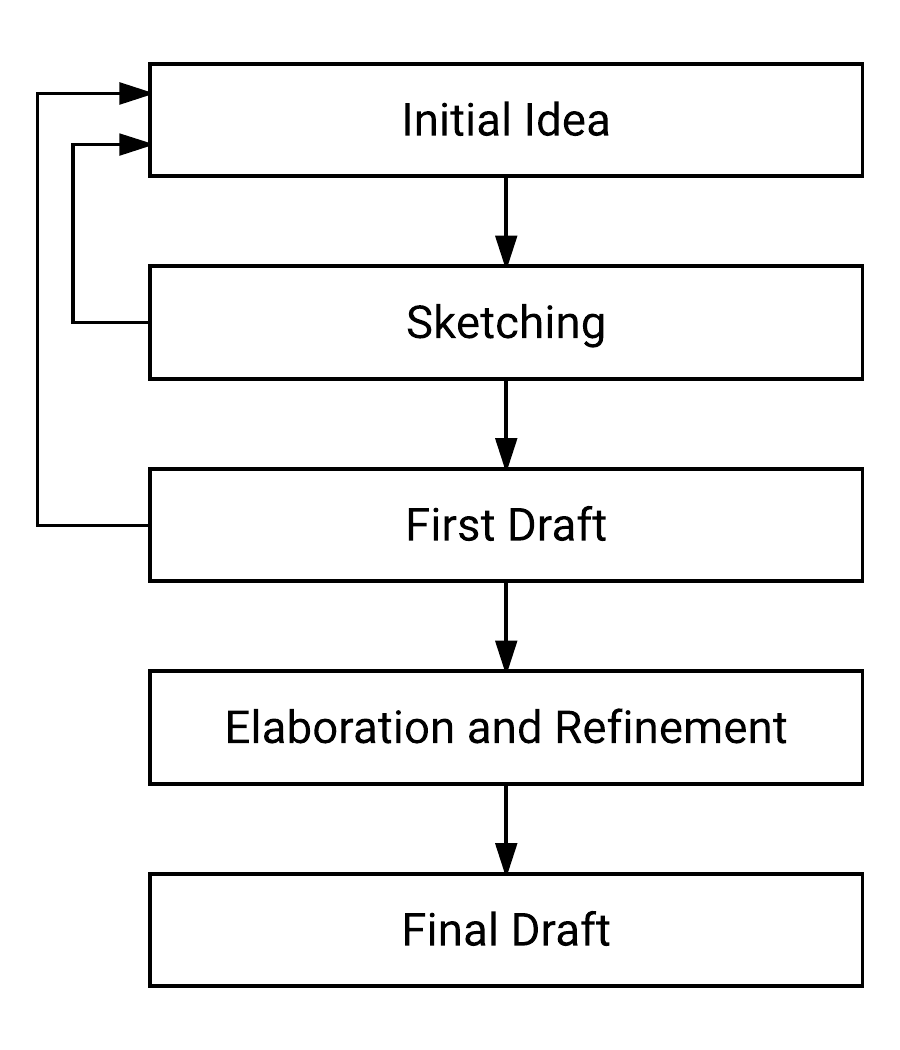
\includegraphics[scale=0.2]{Process_of_Composition}
    		\caption{The stages of music composition. \citep{bennett1976process}} 
    		\label{fig:MUSIC_benettcompositionstages}
		\end{figure}
        \end{comment}
        
        The earlier study of \citet{bennett1976process} reflects the Gestalt theory. It was highlighted in the study that the composition process involved various stages (see Figure \ref{fig:composing-graph}). A composition starts off with a germinal or initial idea for the theme or motif of the composition \citep{bennett1976process,collins2005synthesis}. Once a motif is in mind, the composer moves on to the sketching phase. However, it is still possible for the composer to go back to the ideation stage, even if a draft has already been completed if the composer feels the need for a revision or an unexpected idea comes up. This is what \citet{collins2005synthesis} calls \textit{backtracking}, where the composer goes back to previous stages of the process to reformulate ideas or segments of a draft.
        
        The drafts go through a lot of refinement and revisions as long as the composer is not satisfied with the output \citep{bennett1976process}. Even with the idea in mind, some pieces of the draft might still be improved to better fit the composition. This phase is similar to that of the recurring restructuring stage defined in the study of \citet{collins2005synthesis}. This restructuring involves reformulating pieces of the composition to achieve the final draft. 
        
        % In connection with the Gestalt theory, \citet{bennett1976process} expressed the compositional process in various stages (seen in Figure \ref{fig:MUSIC_benettcompositionstages}) still reflects the Gestalt theory. It starts off at the germinal ideation for the theme or motif from the composer, much like in the process discussed in the study of \citet{collins2005synthesis}, and moves to the sketching period. However the sketching stage and the first draft stage can still go back to the germinal ideation stage for a sudden revision or an unexpected solution encountered by the composer. After the final draft, \citet{bennett1976process} described the last stage of composing as 'Revisions?'. With that said, uncertain or unexpected revisions can be discovered even after the final draft is done. These instances of backtracking can be compared to the recurring restructuring stage from the process discussed by \citet{collins2005synthesis}. It involves reformulating the givens and goals in order to achieve sub-goals. All in all, numerous revisions and restructuring are done in composing music in order to achieve the desired product by the composer.
        

        
        \begin{comment}
      
        %%% Discuss the motif, the main theme of music %%%
        
        Composers often start off with a certain sequence of notes that dictate the theme of their musical composition, this is called the motif. This is the repeating series of notes that occur in different parts of the musical composition. It is also often used to create the last song syndrome (LSS) in most of the songs today.
        
        %%% How the song revolves around the motif using various melodic intervals %%%
        
        From the motif, the composer can then use chord progressions or melodic intervals in order to expand the composition with respect to music theory. However, composers would have to choose those creatively in order to set the mood or emotion that the composition or song wants to portray to listeners.
        
        %%% Mention how composers usually copy paste and transpose or elongate or invert notes %%%
        
        With the recurring theme in the composition, composers are faced with the problem of imitating the motif throughout different parts of the song. Copy pasting is often used in musical notation softwares in order to achieve this. However tweaking through transposing, elongation, or inverting the motif is also evident in order to build variation in delivering the motif in compositions.
        
        \end{comment}
        
        \subsubsection{Concepts}
        
        \paragraph{Fundamentals of Music}
        
        Music cannot be taught without knowing the fundamentals first, namely: pitch and melody, rhythm, texture and harmony, color and timbre, and form or design \citep{rivadelo1986fundamentals}. By combining all of them, they form into what is known today as music \citep{willoughby1971comprehensive}.
        
        %By intertwining them all, it builds into, what we know today, Music \citep{willoughby1971comprehensive}.

Music is mainly formed by several notes or rests in a sequence. A consecutive progression of notes that are relative to each other is called the melody \citep{rivadelo1986fundamentals}. In Paul Hindemith’s theory of melody, melody is considered as the element of a composition that truly reveals the personality of the composer \citep{cheng2016approaching}. 

Pitch is defined as the highness or lowness of a tone or musical sound relative to the amount of vibrations per second \citep{rivadelo1986fundamentals}. Each pitch is represented by the first seven letters in the alphabet, which are A, B, C, D, E, F, and G \citep{miller2005complete}. However, the distance of a pitch from each other can be described as a whole step and a half step or semitone. The distances can be easily derived from the keys of a piano or keyboard. Moving from one key to a next key is called half step or semitone respectively. A whole step on the other hand is described as moving from one key to another by skipping a key between them. Both can be used to traverse forward and backward by adding the word up or down after the distance. Multiple steps can also be achieved by putting a number before the distance.

The pitch can also be represented using the Solfeggio Method, commonly known as the Do-Re-Mi. However, the same pitch representation may also be found on higher or lower tones which are divided by an octave, which is a fixed interval between pitches.

Another element of music is the duration, which is the amount of time a tone lasts \citep{rivadelo1986fundamentals}. The duration is shown in a composition through the use of different notes or rests that indicate the duration of a certain pitch \citep{rivadelo1986fundamentals, burrows1999reading}. More of this will be discussed in Section \ref{sec:musical_notation}.

% Pitch is defined as the highness or lowness of a tone or musical sound which is ascertained by the amount of vibrations per second \citep{rivadelo1986fundamentals}. Each pitch is represented with the first seven letter in the alphabet which is A, B, C, D, E, F, and G \citep{miller2005complete}. They can also be represented using the Solfeggio Method which is commonly known as the Do-Re-Mi. However, the same pitch representation can also be found on higher or lower tones which are divided by an octave which is a fixed interval between pitches.

In a composition, \citet{rivadelo1986fundamentals} mentions that rhythm represents the pace of the musical flow through the common patterns that currently exist. It can be understood as the factor that makes musicians and composers aware of the beat or tempo of composition. It allows them to align their ideas in order to create music on top of the rhythm. 

Rhythm also consists of 4 parts, which are: beat, accent, meter, rhythmic pattern, and phrase \citep{rivadelo1986fundamentals}. The beat is the basic time unit of the composition. The accent forms the theme of the rhythm, while the meter divides the beats into sections. The rhythmic pattern groups the beats to form a coherent pattern of sound. Finally, the phrase is considered as the musical thought, that is a part of the whole musical sentence.

% In a whole composition, \citet{rivadelo1986fundamentals} mentioned that rhythm represents the musical flow’s pace through the common patterns that currently exist. She also stated that “it is the principle that enables one to organize or to bring order into their perception of time and space”. It can be derived that it makes musicians and composers aware of the beat or tempo for them to align with it their ideas in order to create music on top of the rhythm, based on what she said. Rhythm also consists of 4 parts having: beat, accent, meter, rhythmic pattern, and phrase \citep{rivadelo1986fundamentals}. With the beat being the time unit, the accent forming the beats into parts, the meter dividing the beats into sections, the rhythmic pattern grouping the beats to form patterns of sound, and phrase being “the musical thought that is a part of the musical sentence“.



% Consecutive progression of notes that are relative with each other is called Melody \citep{rivadelo1986fundamentals}. In Paul Hindemith’s theory of melody, “melody is the element in which the personal character of the composer is clearly and cleverly revealed” \citep{cheng2016approaching}. Pitch and duration, the amount of time a tone lasts, are the basic properties according to \citet{rivadelo1986fundamentals}. It also has 5 properties that make music different from each other namely: Rhythm, Dimension, Direction or Movement, Progression, and Register. The dimension contains the length and range of a melody. The length, from the term itself, is the measurement of the melody, it can be short or long. The range is the distance of the highest and lowest sound or tone.
        
        \paragraph{Basic Music Theories}
        
        Knowledge of music theory can aid a musician to compose music without having to waste time thinking about succeeding notes or melodies. According to \citet{meyer1989style}, it can be likened to rules or guidelines that can change over time due to changes in cultural style. The theories in music also utilize some of the fundamentals of music to create these guidelines. It assembles the basic fundamentals into a harmonic structure that characterizes and builds music \citep{meyer1989style}.
        
        % Music Theories can aid a musician to compose good music without relying on too much memorization. It can be related to arbitrary rules, as stated by \citet{meyer1989style}, that change over time due to the change in culture. It can also be described to govern music that make songs sound good. The theories in music also utilize some of the fundamentals of music in creating the said arbitrary rules. It assembles the basic fundamentals into a harmonic structure that characterizes and builds into as to what is music today.
        
        There are multiple concepts in music theory that can start off a musician to compose his or her own music piece. Although music theory can serve as a guide for composition, it is not an all-in-one solution. Composers will still have to think creatively to identify which theories are applicable or could be applied in the current composition \citep{meyer1989style}. Some form of trial-and-error would still be present in this process.
        
        %However this may guide the composer in composing music, it is not a all-in-one solution in composing a whole composition. Composers still have to think creatively which theories or part of a theory is most applicable in his or her composition. The trial-and-error process in musical composition would still be present.
        
        Tetrachords are one of the most frequenly used concepts in music theory \citep{spencer1996music}. They are four succeeding notes that form a structure that dictates the perfect fourth of the first note. \citet{spencer1996music} stated 4 kinds of tetrachords: major, minor, natural, and harmonic. They are differentiated by the number of semitones being skipped relevant to the first note. Major follows the pattern 2-2-1 semitones, minor goes 2-1-2, natural uses 1-2-2, and lastly, harmonic follows 1-3-1. 
        
        
        Scales can then be derived from tetrachords \citep{spencer1996music}. Combining two (2) tetrachords and adding a whole step or a tone in the middle of the two tetrachords would result in a scale. For example, two major tetrachords (2-2-1) with a whole step in the middle would result in: 2-2-1-(2)-2-2-1, which is actually the major scale.
        
        %Tetrachords and scales are the first to be discussed by \citet{spencer1996music} as it is going to be used frequently in music theory is a whole. Tetrachords are four succeeding notes that form a structure that dictates the perfect fourth of the first note. \citet{spencer1996music} stated 4 kinds of tetrachords, Major, Minor, Natural, and Harmonic. They are simply explained by showing the number of semitones that you have to skip in order to build the tetrachord based from the first note desired by the composer. Major follows the pattern 2-2-1 semitones, minor goes 2-1-2, natural goes 1-2-2, and lastly, harmonic follows 1-3-1. Scales can be derived with the help of tetrachords. Multiplying two tetrachords and adding a whole step or a tone in the middle of the two semitones forms a scale. For example, two major tetrachords with a whole step or a tone in the middle, 2-2-1-(2)-2-2-1, forms the major scale.
        
        There are certain harmonic intervals that composers can utilize to build a good musical composition \citep{spencer1996music}. These are called melodic intervals. They can be described as various note sequences that composers can use in their composition to build the motif or the whole composition as a whole \citep{spencer1996music}. 
        
        There are two characters used to distinguish intervals from each other. The first character denotes the quality of the interval \citep{spencer1996music}. This can be any of the letters: M, P, m, d, A. M is described as a major interval, P as a perfect interval, m as a minor interval, d as diminished, and A as augmented. Each of these intervals give off different sounds for the note sequences they produce \citep{spencer1996music}.
        
        The second character is about the quantity of an interval. It is a number which identifies the length of the interval or the distance of one note from another \citep{spencer1996music}. However, not all interval qualities contain all interval lengths. Some may contain the same numbers from another melodic interval but they are different in terms of how many semitones are skipped in order to dictate the next note.
        
        % There are certain intervals that are described as harmonic \citep{spencer1996music} that composers can utilize in order to build a good musical composition, they are called melodic intervals. They can be described as various note sequences that composers can use in their composition in order to build the motif or the whole composition as a whole. There are two characters in distinguishing an interval from each other. The first character is the quality of the interval which are the letters, M, P, m, d, A. M is described as a major interval, P as a perfect interval, m as a minor interval, d as diminished, and A as augmented. Each of this interval gives off a different sound when listening to the note sequences it produces. The second character is a number which is the length of the interval or the distance of one note is from the other. However, not all interval qualities contain all interval lengths. Some may contain the same numbers from another melodic interval but they are different in terms of how many semitones are skipped in order to dictate the next note.
 
\begin{comment}

\begin{figure}[H]
\centering
\begin{minipage}{.4\textwidth}
	\centering
	\includegraphics[width=.7\linewidth]{major_triad}
    \caption{Major Triad}
    \label{fig:major_triad}
\end{minipage}
\begin{minipage}{.4\textwidth}
	\centering
	\includegraphics[width=.7\linewidth]{minor_triad}
    \caption{Minor Triad}
    \label{fig:minor_triad}
\end{minipage}
\end{figure}

\begin{figure}[H]
\centering
\begin{minipage}{.4\textwidth}
	\centering
	\includegraphics[width=.7\linewidth]{augmented_triad}
    \caption{Augmented Triad}
    \label{fig:augmented_triad}
\end{minipage}
\begin{minipage}{.4\textwidth}
	\centering
	\includegraphics[width=.7\linewidth]{diminished_triad}
    \caption{Diminished Triad}
    \label{fig:diminished_triad}
\end{minipage}
\end{figure}

\end{comment}

\begin{figure}[H]
	\centering
	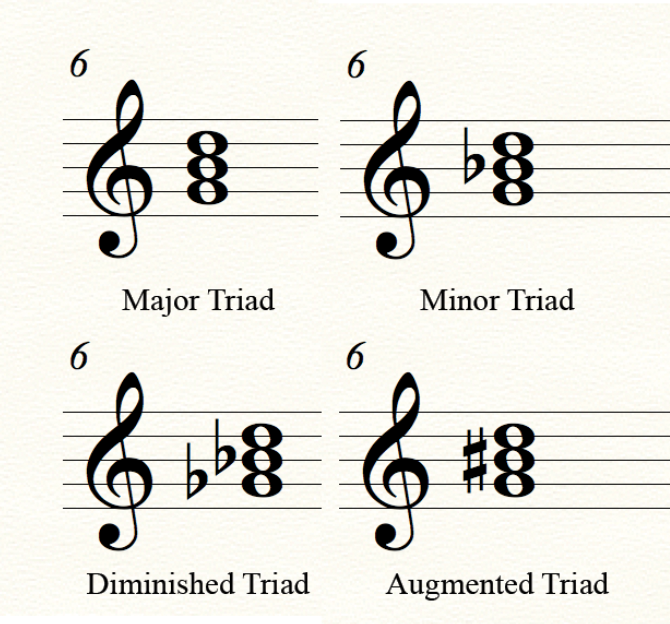
\includegraphics[scale=0.5]{triads}
    \caption{Various triads \citep{spencer1996music}.}
    \label{fig:MUSIC_triads}
\end{figure}
        
        The basic chords in a musical composition are defined by triads. It is basically three notes that are played simultaneously. Like tetrachords, there are four types of triads: major, minor, augmented, and diminished \citep{spencer1996music}. Figure \ref{fig:MUSIC_triads} show the various triads in a musical composition. The lowest note in the triad is called the root, the middle note being the third, and the highest note is called the fifth. However, triads have different qualities in different scales, specifically the major scale, natural minor scale, melodic minor scale, and the harmonic minor scale. In these scales, triads are classified into scale degrees which are like roman numerals which are both lower-case and upper-case. These scale degrees are often used in defining different chord progressions.
        
        
        \paragraph{Musical Notation}
        \label{sec:musical_notation}
        
        The modern notation system in music today, specifically western musical notation, was derived from places where the western culture continued to thrive \citep{read1969music}. However, the practice of writing musical notation did not originate from western culture \citep{read1969music}. Musicologists discovered that pre-Christian Greeks have already been using musical notation, and have developed four (4) unique systems for writing them \citep{read1969music}. Nonetheless, the modern musical notation system holds some similarity to the system developed in the past. 
        
        %The modern notation system in music today, specifically western musical notation, were derived from places where the western culture continued to thrive \citep{read1969music}. However writing musical notations were not originated from the western culture, \citet{read1969music} mentioned that musicologists discovered that pre-Christian Greeks have known musical notation and has four unique systems for writing them. Nonetheless, some resemblances in practice from the past notation system can also be seen in the modern system.
        
        According to \citet{read1969music}, musical notation is known as a method for visually representing musical sound. It is what musicians use to graphically display their musical ideas and can be read by other musicians as well. In relation to writing and reading any character in any language, it also requires understanding of the symbols used in music notation in order to be literate in music \citep{read1969music}. 
        
        %"the visual manifestation of the interrelated properties (or fundamentals) of musical sound". It is what musicians used to graphically display their musical ideas and can be read by other musicians as well. In relation to writing and reading any character in any language, it also requires you to understand the symbols used in music notation in order to be literate in music.
        
\begin{figure}[H]
	\centering
	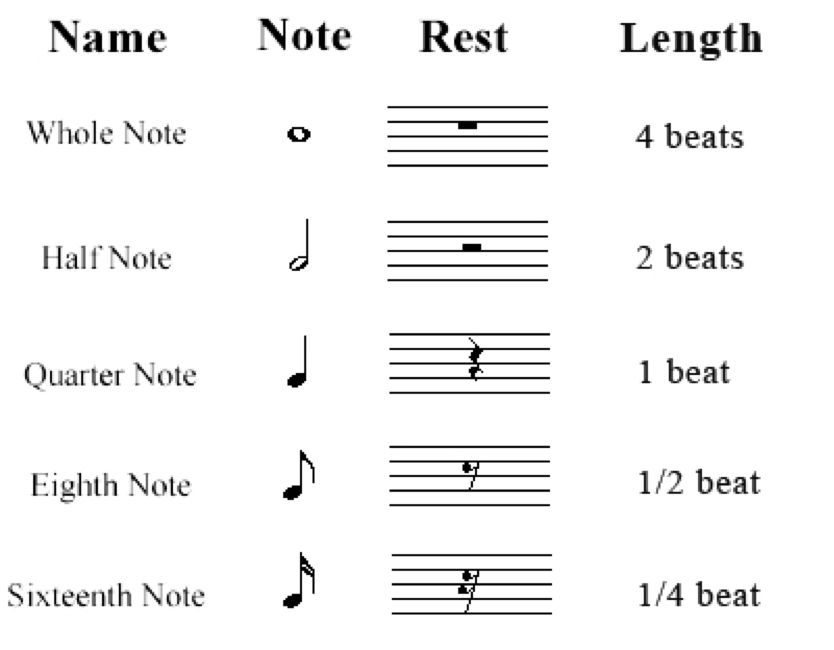
\includegraphics[scale=0.2]{BasicNoteRest}
    \caption{Basic notes and rests used in modern musical notation \citep{riso2016basic}.}
    \label{fig:MUSIC_basic-notes-rests}
\end{figure}
        
        The basic symbols in musical notation are the notes and rests seen in Figure \ref{fig:MUSIC_basic-notes-rests}. These are found throughout the staff, which is the set of lines and spaces that represent the different levels of pitches. Beams are the black bars that are used to group consecutive notes that are less than a quarter note in order to improve the visualization of the composition itself \citep{spencer1996music}. However, the pitches that represent each space or line in the staff is different based on the clef used at the start. The G-Clef or treble clef and the F-Clef or bass clef (see Figure \ref{fig:MUSIC_gclef_fclef}) change the pitch representations on each line and space on the staff. When the G-Clef is used at the start of the staff, each line starting from the bottom represents the pitches E-G-B-D-F and spaces represent the pitches F-A-C-E. On the other hand, when the F-Clef is used at the start of the staff, each line starting from the bottom represents pitches G-B-D-F-A and the spaces represents the pitches A-C-E-G.
        
\begin{figure}[H]
	\centering
	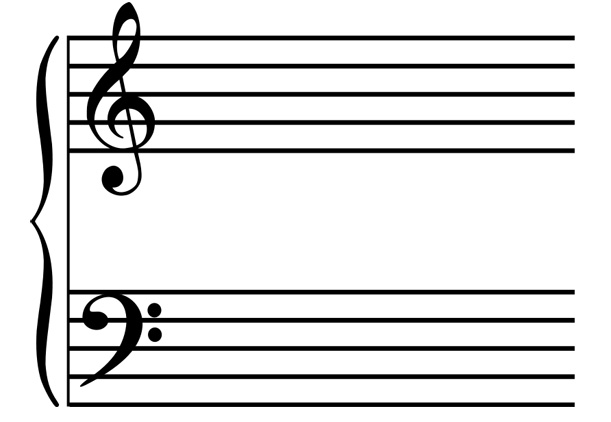
\includegraphics[scale=0.2]{G-ClefAndF-Clef}
    \caption{The G-Clef and F-Clef \citep{stamp2013the}.} 
    \label{fig:MUSIC_gclef_fclef}
\end{figure}

	There is only one element in musical notation that indicates the distinct rhythm throughout the composition, and that is the time signature \citep{rivadelo1986fundamentals}. There are two numbers in the time signature, (see Figure \ref{fig:MUSIC_timesignature}) called the numerator and the denominator. When writing the time signature, the numerator takes up the upper two spaces of the staff while the denominator takes up the lower two spaces of the staff \citep{read1969music}. Each part of the time signature defines the notes to be used in the musical composition. The numerator or the upper number denotes the amount of beats in one bar or measure while the denominator or the lower number indicates the type of note that would equal to one beat \citep{read1969music, rivadelo1986fundamentals,burrows1999reading}.

	% There is one element in musical notation that initializes the distinct rhythm throughout the composition \citep{rivadelo1986fundamentals}, and that is the time signature. There are two numbers in the time signature, seen in Figure \ref{fig:MUSIC_timesignature}, called the numerator and the denominator. In the staff, the numerator takes up the upper two spaces of the staff while the denominator takes up the lower two spaces of the staff \citep{read1969music}. Each part of the time signature defines the notes to be used in the musical composition. According to \citet{rivadelo1986fundamentals}, \citet{read1969music}, and \citet{burrows1999reading}, the numerator or the upper number denotes the amount of beats in a bar or measure while the denominator or the lower number indicates the type of note that would be tantamount to a beat.
    
\begin{figure}[H]
	\centering
	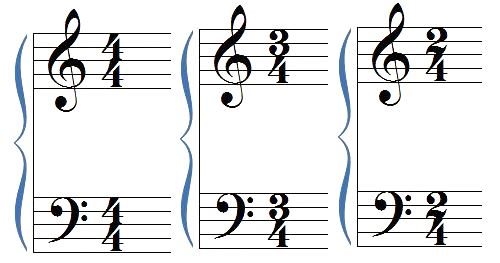
\includegraphics[scale=0.4]{Time-Signature}
    \caption{Various time signatures \citep{rose2014reading}.} 
    \label{fig:MUSIC_timesignature}
\end{figure}

A series of notes in a musical sheet is divided by bar lines (see Figure \ref{fig:MUSIC_barlines}). However, there are two kinds of bar lines in musical pieces. The first is the simple bar line which is one vertical line that divides a series of notes based on the time signature. The second type of bar line is the double bar line which is made up of two vertical lines. It specifies the end of a part in a music composition \citep{read1969music}. This is where composers can change the time signature and key signatures of the current staff. However there are variations to the double bar. The first is the one that signifies the end of the composition which is the ``period'' form \citep{read1969music} or final bar line. This kind of bar line is found at the end of the composition. The other two variations are double bars that work together, they are the start repeat and the end repeat. It encloses a number of bars between the start and end repeat which sums up the number of beats as a whole that would satisfy the time signature declared before the start repeat bar.
    
\begin{figure}[H]
	\centering
	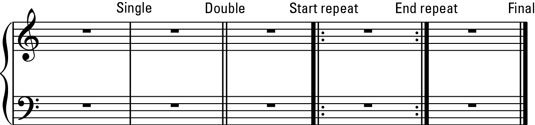
\includegraphics[scale=0.4]{barlines}
    \caption{The different bar lines \citep{dummy2017barlines}.} 
    \label{fig:MUSIC_barlines}
\end{figure}

There are certain annotations that are used to dictate the strength of the sound of notes, these are called dynamics. Shown in Figure \ref{fig:MUSIC_dynamic} are several levels of dynamics that can be used in musical compositions. These markings can be usually found above or below the notes that are affected by the dynamic marking \citep{read1969music}. However, there are symbols that also complement dynamic markings, which are called dynamic signs. 

Crescendo and diminuendo or decrescendo are the only dynamic signs. Both signs are used when a succession of notes is gradually increasing or decreasing to a certain dynamic. The example shown in Figure \ref{fig:MUSIC_dynamicsignsmarkings} exhibits the use of both signs. Basically, crescendo is when the loudness increases up to a certain dynamic and decrescendo is when the loudness decreases down to a certain dynamic. In Figure \ref{fig:MUSIC_dynamicsignsmarkings}, crescendo is used when the loudness of the notes increased from mezzo forte to forte. Decrescendo is used when the loudness of the notes descended from forte to mezzo forte.

	% There are certain annotations that are used in order to dictate the strength of sound of the notes, it is called dynamics. In Figure \ref{fig:MUSIC_dynamic}, there are several levels of dynamics that can be used in musical compositions. These markings can be usually found above or below the notes that are affected by the dynamic marking \citep{read1969music}. However, there are symbols that also complement dynamic markings which are dynamic signs. Crescendo and diminuendo or decrescendo are the only dynamic signs. Both signs are used when succession of notes are gradually increasing or decreasing to a certain dynamic. An example in Figure \ref{fig:MUSIC_dynamicsignsmarkings} exhibits the use of both signs. Basically, crescendo is when the loudness increases up to a certain dynamic and decrescendo is when the loudness decreases down to a certain dynamic. From Figure \ref{fig:MUSIC_dynamicsignsmarkings}, crescendo is used when the loudness of the notes increased from mezzo forte to forte. Decrescendo is used when the loudness of the notes descended from forte to mezzo forte.
    
\begin{figure}[H]
	\centering
	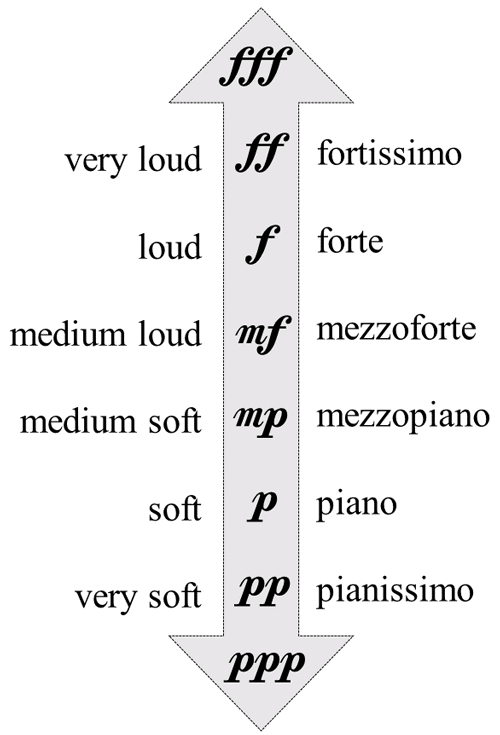
\includegraphics[scale=0.2]{dynamic_markings}
    \caption{The various dynamic markings \citep{peter2016dynamic}.}
    \label{fig:MUSIC_dynamic}
\end{figure}

\begin{figure}[H]
	\centering
	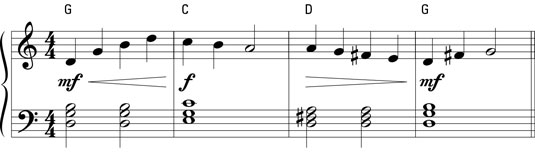
\includegraphics[scale=0.4]{dynamic_signsandmarks}
    \caption{Dynamic markings and signs \citep{dummy2016volume}.}
    \label{fig:MUSIC_dynamicsignsmarkings}
\end{figure}
 
        \paragraph{Circle of Fifths}
        
\begin{figure}[H]
	\centering
	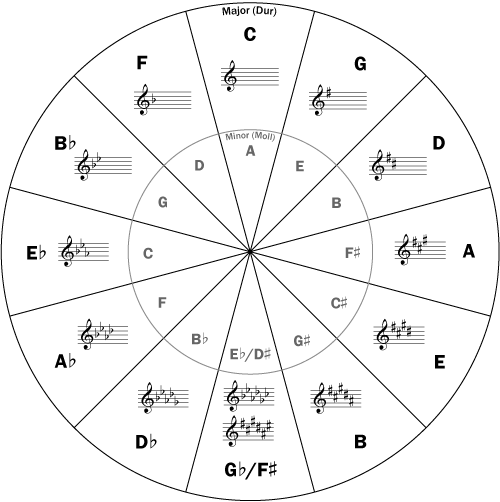
\includegraphics[scale=0.5]{circle-of-fifths}
    \caption{The circle of fifths \citep{gleaves2015understanding}.}
    \label{fig:MUSIC_circleoffifths}
\end{figure}
        
        The circle of fifths (see Figure \ref{fig:MUSIC_circleoffifths}) was derived from the the Pythagoras Circle made by famous Greek philosopher Pythagoras \citep{jensen1992circle}. It was later expanded in the work of Nikolai Diletskii on amplification and Johann Heinichen's work on modulation \citep{jensen1992circle}. It is also now commonly used today as a basis for teaching techniques in composing and playing music. Some of these techniques include modulation and chord progressions. %Nonetheless, the circle of fifths requires a few amounts of time in order to learn how to read and utilize it.
        
         It can be compared to a 12-hour round clock with the numbers replaced by the names of different pitches (see Figure \ref{fig:MUSIC_circleoffifths}). All of the succeeding pitch representations going clockwise starting from C are derived from the fifth of the previous pitch \citep{jensen1992circle}. For example, starting from C, the fifth of C would be G, and the fifth of G would be D and so on. It would revolve back to C when it reaches F. The inner circle is a copy of the outer circle only moved counter-clockwise twice.
        
       % It can be compared to a 12-hour round clock with the numbers replaced by the names of different pitches. Each number in the clock also represents a pitch representation as seen in Figure \ref{fig:MUSIC_circleoffifths}. All of the succeeding pitch representations, clockwise from C, is derived by the fifth of the previous pitch. For example, starting from C, the fifth of C would be G, and the fifth of G would be D and so on. It would revolve back to C when it reaches F. The inner circle is a copy of the outer circle only moved counter-clockwise twice.
        
        Although it may look like a clock, counting with the circle of fifths is different. It starts at 0 from the top or north and both sides (clockwise and counter-clockwise) count from 1 and end at 6 at 6 o'clock. Those numbers denote the key signatures that are present in a major or minor scale in a musical composition \citep{jensen1992circle}. Key signatures are derived from the circle of fifths through the counting. The sharps in the key signature begin counting clockwise at F and flats begin counting counter-clockwise at B \citep{clough1986musical}.
        
        %Although it may look like a clock, counting with the circle of fifths is different as it starts at 0 from the top or north and both sides (clockwise and counter-clockwise) counts from 1 and ending at 6 at 6 o'clock. Those numbers denote the key signatures that are present in a major or minor scale in a musical composition. Key Signatures are derived from the circle of fifths with the help of counting with the use of the numbers. The sharps in the key signature begin counting clockwise at F and flats begin counting counter-clockwise at B.
        
        %%% Discuss how chords are derived from the circle %%%
        
        From the circle of fifths, major triads can be derived \citep{jensen1992circle, spencer1996music}. This can be done by choosing a root note from the outer circle, then getting its third and fifth \citep{jensen1992circle}. The third can be found by traveling four (4) semitones, or two (2) tones clockwise from root note. The fifth can be easily found by looking at the note next to the root note, clockwise. For example, if C is chosen as the root note, the third, which is four (4) semitones clockwise from C, would E, and the fifth would be G, which is just next to C.
        
        Minor triads can also be found in the circle of fifths but through a different way compared to deriving major triads \citep{jensen1992circle}. Again, the root is chosen from the outer circle. The third is found by moving three semitones counter-clockwise from the root. The fifth is taken similarly to how it is taken in major triads, just get the note next to the root note, clockwise. Similar to the previous example, C will be chosen as the root note. In this case, its third would be E minor, which is three semitones counter-clockwise to C. The fifth in this triad would be G. 
        
        
        % With the circle of fifths, triads can be derived. The inner circle of the circle of fifths is also used in deriving the triads. The way of finding a major triad is you choose a root note from the outer circle and then the third and the fifth can be found by looking at the note right next to the root note clockwise. The third is simply the pitch parallel in the inner circle of the fifth. For example, choosing C as the root note, G would be the fifth and A would be the third. However, minor triads can also be found in the circle of fifth but with a different way compared to deriving major triads. In choosing the root for a minor triad, the inner circle is used. From there we get the pitch that is parallel to it from the outer circle and that is the third. Lastly, the fifth is the pitch right next to the root counter-clockwise in the inner circle. For example, choosing A as the root note, C would be its third, and E would be the fifth. From the major and minor triads, different triads can also be discovered by adjusting the third or root note to suit the other triads.
        
        %%% Discuss modulations used %%%
		
        The circle of fifths can also be used in modulation from different scales \citep{clough1986musical,jensen1992circle}. One event where modulation would be needed is when a composition needs to fit the singer's vocal range and key. Using the key signatures derived from the circle of fifths, composers can easily transpose the key signatures of composition. % needs to be edited
        
        % Modulating from different scales can also be aided with the help of the circle of fifths. A good example for the use of modulating is when compositions are needed to be modulated in order to suit a certain singer's vocal range and unique key. With the given key signatures in the circle of fifths, composers could alter a composition easily by modulating through the circle of fifths based on the current key they composition have to a another key.
        
        
        \subsubsection{Musical Metacreation}
            
            For a long time, artificial intelligence has mainly been used in pursuing problem solving and mathematical and analytical applications \citep{steels1993artificial}. However, with its growing possibilities, artificial intelligence has seen applications in several domains such as speech, image recognition, and even creative endeavors \citep{russell1995modern}. Computational creativity, is a form of artificial intelligence with a focus on understanding and modeling the creative human brain \citep{pasquier2017an}. 
            
            The subfield of computational creativity, musical metacreation, is mainly concerned with the study of endowing or giving machines the capacity to perform and undergo creative musical tasks like composition or interpretation  Musical metacreation can be done through several algorithms or techniques. In the study of \citet{tokui2000music}, \citet{birchfield2003generative}, and \citet{kikuchi2014automatic}, genetic algorithms were used to metacreate melodies and rhythms, while \citet{geis2008creating} used an Ant Colony Optimization algorithm to account for the variances that composers add to their composition. 
            
            However, given the limited time allowed in this study, the researchers opted to use a rule-based algorithm in favor of the other algorithms.
        
        	\paragraph{Rule-based Algorithms}
            	
                The goal of the study of \citet{bozhanov2014computoser} was to improve on the limitations and alleviate problems present in other algorithms such as the lack of a user interface, the composition's pleasantness, but more specifically, the lack of variation. The result of this study was Computoser, a probabilistic rule-based musical metacreation algorithm. When composing music, Computoser follows a set of rules coming from music theory. Additionally, since the algorithm is a hybrid between probability-driven and rule-based, Computoser attaches probabilities to these rules, for example in the set of notes that can be generated (Table \ref{tab:cnp}), ensuring that there is variation between the compositions \citep{bozhanov2014computoser}. 


\begin{table} [!htbp]  
\centering
        \captionof{table}{Computoser Note Probability \citep{bozhanov2014computoser}}\label{tab:cnp}
   \vspace{0.20cm}    
        \begin{tabular}{|p{4cm}|p{2cm}|} %{|l|l|l}
        \hline 
       Note & Probability \\ \hline
       Sixteenth & 10\% \\ \hline
       Eighth & 31\% \\ \hline
       Quarter & 40\% \\ \hline
       Dotted Quarter & 7\% \\ \hline
       Half & 9\% \\ \hline
       Whole & 3\% \\ \hline
        \end{tabular}
\end{table}

The core of the Computoser algorithm comes from its rules \citep{bozhanov2014computoser}. The algorithm has rules on the following:

\begin{itemize}
\item Structure
\item Rhythm
\item Repetition
\item Variations
\item Dissonance and syncopation
\item Endings
\item Effects
\end{itemize}

The most interesting of these, is the variation. Variations prevent music from becoming boring, yet still allow some form of repetition \citep{kivy1993fine,bozhanov2014computoser}. Because the goal of the study was to improve on the lack of variation in other algorithms, Computoser allowed several kinds of variations in its compositions whenever needed, which on average was found to be after every 2 measures \citep{bozhanov2014computoser}. 

The variations present in Computoser that will also be used in this study are: transposition, inversion, and retrograding. Transposition is done by simply moving a set of notes to a different scale, either lower or higher \citep{owens1998composers}. Inversion is done by reversing the notes on a horizontal axis or in layman's terms, turning them upside down based on a scale while keeping their intervals \citep{owens1998composers}. On the other hand, retrograding is done by reversing the notes on a vertical axis, or basically playing them backwards \citep{owens1998composers}. These variations will be used in the proposed system to allow composers to alter a set of notes but maintain some similarity or resemblance to the original set of notes.

Another rule-based musical metacreation algorithm is the one developed in the study of \citep{schulze2011music}. The result of the study was SuperWillow, a system whose aim was to generate music that were pleasurable to the human ear. The system used probabilistic automata and Markov chains built by analyzing music data to generate its music. 

SuperWillow was built by analyzing music data in the form of a MusicXML file \citep{schulze2011music}. Because the data was in this format, it was easy for them to retrieve information like the tempo, scale, and time signature. The analyzed data was used to generate analysis objects: Markov chains which can be used to model a sequence of tasks or events through states. Markov chains satisfy the Markov assumption, which states that: 

\begin{equation}
P(q_t|q_{t-1},q_{t-2},...,q_1) = P(q_t|q_{t-1})
\end{equation}

		$q_1,...,q_t$ are a set of states, while $t$ is the time. What this algorithm means is that the transition of each state must not depend on previous states, and only depend on the current state \citep{schulze2011music}. 
        
        These analysis objects are then used when generating music to imitate the styles of the music that was used as input \citep{schulze2011music}. Musical styles can be generated randomly or chosen by the user from the list available from the input. Following this, other important musical information is selected randomly, again from the set of input music. The specific Markov chains for generating the chord progression and rhythm are then used to generate the set of notes that will be played \citep{schulze2011music}. 
        
        The music generated by SuperWillow were evaluated through a partial Turing test by making 263 respondents, composed of professors and students from Stellenbosch University, listen to a mix of both human composed music and the generated music by SuperWillow \citep{schulze2011music}. The results of the survey were promising, showing that 38\% of the respondents thought that the music composed by SuperWillow was composed by a human. Given this, the researchers are still aiming to add to the capabilities of SuperWillow by improving how it analyzes the training data \cite{schulze2011music}. The system can be found at \url{http://superwillow. sourceforge.net}.
        
	\subsection{Existing Systems}
        \subsubsection{komp}
        
        ``\textit{komp}'' is a musical composition application for the iOS platform developed by Semitone \citep{macdonald2017komp}. komp promotes the natural way of musical notation, given that its method of input is by drawing notes on a digital music sheet. The drawn note would then be recognized by the application's built-in image recognition model, and rendered as a digital note. However, the main drawback of this method is that the faulty image recognition is an annoyance or obstruction to composition \citep{macdonald2017komp} 
        
        %"komp" is a musical composition iOS application developed by S\'emitone with members from their team that has experience in music and design. It promotes the natural way of writing down notes in a piece of paper by requiring the user to input notes via drawing them into the musical sheet present in the application. However, input recognition may seem to obstruct the process in inputting the notes.
        
        Drawing notes into the musical sheet may seem natural but it can be obtrusive in some instances \citep{macdonald2017komp}. Sometimes the recognition of the location of the drawing may bug out and place notes in places that the user did not desire. The recognized note from the drawing may also be wrong during some instances which results in wasted time erasing the generated note \citep{macdonald2017komp}. 
        
        This application presents a solution to this problem by allowing users to use their built-in learning tool. The tool requests users to draw a specified note multiple times to better learn how the user draws the note and adjust the image recognition model to suit the user's style \citep{macdonald2017komp}. 
        
        Although this looks like a good solution, the application still has limitations. According to \citet{macdonald2017komp}, the handwriting feature cannot detect sixteenth rests or notes. This could still be remedied using the built-in learning tool but the user would have to create their own way of writing the sixteenth note or rest in order for it to be possible. This solution would then remove the naturalness of the input method because composers would have to write sixteenth notes or rests differently from it is actually written \citep{macdonald2017komp}.
        
        %Drawing notes into the musical sheet may seem natural but it can be obtrusive in some instances. Sometimes the recognition of the location of the drawing may bug out and place notes in places that the user did not desire. The recognized note from the drawing may also be wrong at some instances which may result into repetitive erasing \citep{macdonald2017komp}. This may be remedied with their built-in learning tool where the user inputs a number of their drawings for each note and the application learns that drawing to make the drawing recognition suited for the user. Although this looks like a good solution, this solution can hinder flexibility for users that use the same application in the same device. Some composers may differ in their style of drawing notes into komp and would definitely affect the recognition. According to \citet{macdonald2017komp}, there are also limitations to the handwriting feature in a way that sixteenth rest note or a triplet cannot be inputted through handwriting. However, this can also be remedied with the built-in learning tool but you have to create your own way of writing the sixteenth note in order for it to be possible.
        
    	\subsubsection{Finale}
        
        Finale is a musical notation software that is available for both the Windows and macOS platforms. It is widely known for its large set of features or functions such as keyboard shortcuts \citep{knoder2017finale} and the speedy entry tool that can make musical notation faster. It also uses MusicXML files to store and share compositions with other composers, or for use in other musical notation software that support MusicXML \citep{otter2017finale}.
                
        % Finale is a musical notation software that is available for both the Windows and macOS platforms. It uses MusicXML files in order to save or share music compositions through other musical notation software that also support MusicXML \citep{otter2017finale}. It is widely known for its wide-range set of features or functions such as keyboard shortcuts \citep{knoder2017finale} and the speedy entry tool that can ease the musical composition process.
        
        Finale allows composers to drag notes or rests to the music sheet. This presents an easy method of adding notes to the sheet \citep{otter2017finale}. However for expert users, Finale allows the use of keyboard shortcuts to speed up musical notation. Notes are assigned to specific number key on the keyboard, so adding a note to the music sheet can be as simple as pressing a key \citep{knoder2017finale}. This method saves time from having to find the right note or rest and dragging it to the music sheet. Although it might not feel natural for musical composers that are used to writing musical notes on paper, it is faster \citep{knoder2017finale}. 
        
        %Copying and pasting is also made easy with the use of keyboard shortcuts, however only on macOS. A user can simply highlight his or her desired selection that he or she wishes to copy and paste and holds down the option key and clicks on the desired location that he or she desires to paste the highlighted selection.
        
        %Keyboard shortcuts in Finale are commonly used in order to speed up writing musical notes into the music sheet. As simple as pointing the indicator in the musical staff and pushing down number keys in the keyboard and then it will then output a corresponding note that is assigned to the number key \citep{knoder2017finale}. It saves time in finding the right the musical note by dragging and dropping it into the musical sheet itself. Although it might not feel natural for musical composers that are used to writing musical notes on paper, it is faster. Copy and pasting is also made easy with the use of keyboard shortcuts, however only on macOS. A user can simply highlight his or her desired selection that he or she wishes to copy and paste and holds down the option key and clicks on the desired location that he or she desires to paste the highlighted selection.

		Finale's speedy entry tool works hand-in-hand with the application's keyboard shortcuts. The tool changes the default indicator found in the staff and replaces it with a box that has a small black block indicating which space or line is currently selected. The block can be moved up or down to change the selected space or line by pressing the up and down arrow keys respectively. When combined with the shortcut for note input, the application allows composers to write compositions faster \citep{knoder2017finale}.
		
        
       % There is another tool used in Finale that works hand in hand with keyboard shortcuts, it is called the speedy entry tool. It changes the default indicator found in the staff and replaces it with a box that has a small black block indicating which space or line is currently selected. The block can be moved up or down to change the selected space or line in the staff with the up and down arrow keys. Combined with the keyboard shortcut that places notes via the number keys, it is easy to input a note to your desired location.
        
		\subsubsection{Sibelius}
        
        Sibelius is another musical notation software that is also available for both Windows and macOS machines. However, compared to Finale, Sibelius offers less keyboard shortcuts and an overloaded interface with too many options \citep{hess2008sibeliusvsfinale}. Despite this, Sibelius still proves to be a viable option for musical composition on computers \citep{knoder2017sibelius}.
        
        %Sibelius is another musical notation software that is also available for both Windows and macOS machines. However compared to Finale, the easing of the composition process is not evident due to less keyboard shortcuts and a user interface that presents too much options that hinders getting things done \citep{hess2008sibeliusvsfinale}. However, it is still a viable option for composing music with the aid of computers.
        
        Sibelius requires users to input notes by selecting a note from the floating menu, and clicking on the desired location in the staff. Unlike Finale, Sibelius does not support keyboard shortcuts for faster note input \citep{knoder2017sibelius}. This task proves to be too heavy for longer compositions, and is a burden for expert users \citep{hess2008sibeliusvsfinale}. However, this method is helpful for beginner composers because of its simplicity.
        
        % Unlike Finale's way of easily inputting notes into the musical sheet, Sibelius requires you to click the note from their provided floating menu, specifically the keypad, and click on the desired location in the staff. Despite it being task heavy for inputting many notes, it is helpful for beginner composers that are not that familiar with the look of notes. The actions in placing notes may be simple but it is going to be task heavy when the user decides to input many varying notes.
        
        An interface that presents too many options or features may be good for people that like to explore and learn the software, but it may be obtrusive for some users that wish to learn the software with minimal exploration \citep{galitz2007essential}. However, Sibelius presents an organized set of options by separating them into sorted tabs. This makes it easier for users to find what they are looking for \citep{hess2008sibeliusvsfinale}. The menus are also designed in a way that it looks like the menus present in Microsoft Office 2007 and recent versions.
        
        %An interface that presents too many options or features may be good for people that like to explore and learn the software, but it may be obtrusive for some users that wish to learn the software with minimal exploration \citep{galitz2007essential}. However, Sibelius presents an organized set of options in which they are sorted by tabs that make it easy for users to find what they are looking for. The menus are also designed in a way that it looks like the menus present in Microsoft Office 2007 and recent versions.

\begin{comment}

\end{}

\section{Music Theory}

\subsection{Fundamentals of Music}

As stated by Rivadelo (1986), music cannot be taught without knowing the fundamentals first namely: Pitch and Melody, Rhythm, Texture and Harmony, Color and Timbre, and Form or Design. By intertwining them all, it builds into, what we know today, Music (Willoughby, 1971).

Pitch can be easily defined as the highness or lowness of a tone or musical sound which is ascertained by the amount of vibrations per second (Rivadelo, 1986). Say for example, %TODO continue with more musical terms

In a whole composition, Rivadelo (1986) mentioned that rhythm represents the musical flow’s pace through the common patterns that currently exist. She also stated that “it is the principle that enables one to organize or to bring order into their perception of time and space”. It can be derived that it makes musicians and composers aware of the beat or tempo for them to align with it their ideas in order to create music on top of the rhythm, based on what she said. Rhythm also consists of 4 parts having: beat, accent, meter, rhythmic pattern, and phrase (Rivadelo, 1986). With the beat being the time unit, the accent forming the beats into parts, the meter dividing the beats into sections, the rhythmic pattern grouping the beats to form patterns of sound, and phrase being “the musical thought that is a part of the musical sentence“.

Consecutive progression of notes that are relative with each other is called Melody (Rivadelo, 1986). In Paul Hindemith’s theory of melody, “melody is the element in which the personal character of the composer is clearly and cleverly revealed” (Cheng, 2016). Pitch and duration, the amount of time a tone lasts, are the basic properties according to Rivadelo (1986). It also has 5 properties that make music different from each other namely: Rhythm, Dimension, Direction or Movement, Progression, and Register. The dimension contains the length and range of a melody. The length, from the term itself, is the measurement of the melody, it can be short or long. The range is the distance of the highest and lowest sound or tone.

\subsection{Musical Notation}

%% Describe each part of the staff in music notation

\subsection{The Circle of Fifths}

The Circle of Fifths was derived from the the Pythagoras Circle made by famous Greek philosopher Pythagoras. It was later expanded by the work of Nikolai Diletskii on amplification and Johann Heinichen's work on modulation \citep{jensen1992circle}. It is also now commonly used today as a basis in teaching techniques in composing and playing music. Some simple techniques include, modulation and chord progressions. Nonetheless, the circle of fifths requires a few amounts of time in order to learn how to read it.

\section{Musical Metacreation}

%%I think we need more components separately defined for each part in the music generation


\subsection{Prediction Suffix Automata}

The theories discussed will be used to define the set of rules that will be needed in the implementation of the system. The rules will serve as the logic behind the music metacreation. The states that will be generated by the Prediction Suffix Automata (PSA) will represent the different possible sequence of notes. The defined rules will be applied to generate these possible sequences of notes. Each state will have an assigned probability to produce a more varied sequence of notes that still follows the rules that were defined. Prediction Suffix Automata (PSA) will be used to model the sequence of notes which will be adapted from the work of \citet{merwe2011music}. PSA is defined as a 4 - tuple $\langle\Sigma, Q, \tau, p\rangle$ where:

\begin{itemize}
	\item $\Sigma$ is the finite input alphabet;
  	\item Q is a set of hidden states;
  	\item a: Q x Q $\rightarrow$ [0, 1] is a mapping defining the probability of transitions between hidden states;
  	\item b: Q x $\Sigma \rightarrow$ [0, 1] is a mapping defining the emission probability of each visible symbol at a given hidden state, also called a confusion
matrix;
  	\item $\pi$: Q $\rightarrow$ [0, 1] is a mapping that defines the initial probability of the hidden states.
\end{itemize}

The following constraints are applied:

\begin{itemize}
	\item $\Sigma_{\sigma\epsilon\Sigma}$p(q, $\sigma$) = 1 for all q $\epsilon$ Q;
    \item the start state $q_0$ is the empty string $\lambda$; and
    \item for all q $\epsilon$ Q and $\sigma$ $\epsilon$ $\Sigma$, $\tau$(q, $\sigma$) is equal to the longest suffix of q$\sigma$ that is in Q.
\end{itemize}

In the work of \citet{merwe2011music}, the LearnPSA algorithm was used in order to generate the transition states given two input note sequences. However, in this study no machine learning algorithms will be used, instead, a rule - based technique will be implemented to allow more time in improving the user experience of the application.

\section{Gesture Interaction}

The study of gesture interactions is rooted in \textit{semiotics}, which are the factors related to the interpretation of different signs and symbols in different languages \citep{kammer2010towards,eco1976theory,nespoulous2014biological}. 

% Migo's gesture stuff

% How does decided platform recognize gestures
The application's selected platform iOS, recognizes gestures through the \texttt{UIGestureRecognizer} class, implemented in the Swift programming language. This class is the one that detects gestures and passes them to other related objects that would act on that gesture. An important thing to note is that it does not perform anything related to the gestures, it only passes them. This was done in order to decouple the logic for recognizing the gesture and acting on it \citep{apple2017ui}.

By default, the \texttt{UIGestureRecognizer} class allows the detection of common gestures like taps, holds, pinchs, and more through its subclasses. It communicates with \texttt{UIGestureRecognizerDelegate} classes to better control gestures in applications. The way gestures work in iOS is that the window or view reads the gestures and checks if any \texttt{UIGestureRecognizer} object recognizes the gesture performed. If one does, it would then pass control to that object. 

% How does gesture generate the notes

In the proposed system, gesture plays an important role in the musical metacreation; as it is the method of input that decides which rules to follow when generating the sequence of notes. h

\end{comment}